\begin{document}

\frontmatter
\title{GLIMMER Documentation}
\author{Magnus Hagdorn\thanks{Magnus.Hagdorn@ed.ac.uk}, Ian
  Rutt\thanks{I.C.Rutt@bristol.ac.uk} and Tony Payne\thanks{A.J.Payne@bristol.ac.uk}}
\maketitle
\tableofcontents

\mainmatter
\chapter{User Guide}
\newcommand{\dir}{ug}
\newcommand{\dir}{ug}

\pagestyle{myheadings}
\markright{GLIMMER 1.0 user documentation}

\begin{document}
\title{GLIMMER 1.0 User Documentation}
\author{Magnus Hagdorn\thanks{Magnus.Hagdorn@ed.ac.uk}, Ian
Rutt\thanks{I.C.Rutt@bristol.ac.uk} \and Tony Payne\thanks{a.j.payne@bristol.ac.uk}}
\maketitle
\tableofcontents
\newpage

\newcommand{\dir}{ug}

\pagestyle{myheadings}
\markright{GLIMMER 1.0 user documentation}

\begin{document}
\title{GLIMMER 1.0 User Documentation}
\author{Magnus Hagdorn\thanks{Magnus.Hagdorn@ed.ac.uk}, Ian
Rutt\thanks{I.C.Rutt@bristol.ac.uk} \and Tony Payne\thanks{a.j.payne@bristol.ac.uk}}
\maketitle
\tableofcontents
\newpage

\newcommand{\dir}{ug}

\pagestyle{myheadings}
\markright{GLIMMER 1.0 user documentation}

\begin{document}
\title{GLIMMER 1.0 User Documentation}
\author{Magnus Hagdorn\thanks{Magnus.Hagdorn@ed.ac.uk}, Ian
Rutt\thanks{I.C.Rutt@bristol.ac.uk} \and Tony Payne\thanks{a.j.payne@bristol.ac.uk}}
\maketitle
\tableofcontents
\newpage

\input{\dir/ug.tex}
\appendix
\section{netCDF Variables}
\input{\dir/varlist.tex}
\end{document}
\appendix
\section{netCDF Variables}
%%%%%%%%%%%%%%%%%%%%%%%%%%%%%%%%%%%%%%%%%%%%%%%%%%%%%%%%%%%%%%%%%%%%%%%%%%%%%%%%
% WARNING: this file was automatically generated on
% Tue, 11 Jan 2005 15:56:57 +0000
% from varlist.tex.in
%%%%%%%%%%%%%%%%%%%%%%%%%%%%%%%%%%%%%%%%%%%%%%%%%%%%%%%%%%%%%%%%%%%%%%%%%%%%%%%%

\label{ug.sec.varlist}
The following list shows all the variable names used by GLIMMER. Only variables marked with $^\ast$ are loaded by the input routines. Append \texttt{\_spot} to the variable name to get single location version of the variable.
\begin{center}
    \tablefirsthead{%
    \hline
        Name&  Description & Units\\
    \hline
    \hline}
  \tablehead{%
    \hline
    \multicolumn{3}{|p{0.98\textwidth}|}{\emph{\small continued from previous page}}\\
    \hline
        Name&  Description & Units\\
    \hline
    \hline}
  \tabletail{%
    \hline
    \multicolumn{3}{|r|}{\emph{\small continued on next page}}\\
    \hline}
  \tablelasttail{\hline}
  \begin{supertabular}{|l|p{8cm}|c|}
    \hline
\texttt{ablt} & ablation & meter/year\\
\hline
\texttt{acab} & accumulation, ablation rate & meter/year\\
&CF name: \texttt{land\_ice\_surface\_mass\_balance}&\\
\hline
\texttt{arng} & annual temperature range & degree\_Celcius\\
\hline
\texttt{artm} & annual mean air temperature & degree\_Celcius\\
&CF name: \texttt{surface\_temperature}&\\
\hline
\texttt{bmlt} & basal melt rate & meter/year\\
&CF name: \texttt{land\_ice\_basal\_melt\_rate}&\\
\hline
\texttt{btemp} & basal ice temperature & degree\_Celcius\\
\hline
\texttt{btrc} & basal slip coefficient & meter/pascal/year\\
\hline
\texttt{bwat} & basal water depth & meter\\
\hline
\texttt{diffu} & apparent diffusivity & meter2/year\\
\hline
\texttt{dusrfdtm} & rate of upper ice surface elevation change & meter/year\\
\hline
\texttt{flwa} & ?? & ??\\
\hline
\texttt{lat}$^\ast$ & Latitude & degreeN\\
&CF name: \texttt{latitude}&\\
\hline
\texttt{lon}$^\ast$ & Longitude & degreeE\\
&CF name: \texttt{longitude}&\\
\hline
\texttt{lsurf} & ice lower surface elevation & meter\\
\hline
\texttt{mask}$^\ast$ & upscaling and downscaling mask & 1\\
\hline
\texttt{prcp} & precipitation & meter/year\\
&CF name: \texttt{lwe\_precipitation\_rate}&\\
\hline
\texttt{presprcp}$^\ast$ & present day precipitation & meter/year\\
\hline
\texttt{presusrf}$^\ast$ & present day surface of the ice-sheet & meter\\
\hline
\texttt{relx}$^\ast$ & relaxed bedrock topography & meter\\
\hline
\texttt{std\_dev}$^\ast$ & standard deviation of sub-grid topography & meter\\
\hline
\texttt{temp} & ice temperature & degree\_Celcius\\
&CF name: \texttt{land\_ice\_temperature}&\\
\hline
\texttt{thk} & ice thickness & meter\\
&CF name: \texttt{land\_ice\_thickness}&\\
\hline
\texttt{topg}$^\ast$ & bedrock topography & meter\\
&CF name: \texttt{bedrock\_altitude}&\\
\hline
\texttt{ubas} & basal slip velocity in x direction & meter/year\\
&CF name: \texttt{land\_ice\_basal\_x\_velocity}&\\
\hline
\texttt{uflx} & flux in x direction & meter2/year\\
\hline
\texttt{usurf}$^\ast$ & ice upper surface elevation & meter\\
\hline
\texttt{uvel} & ice velocity in x direction & meter/year\\
&CF name: \texttt{land\_ice\_x\_velocity}&\\
\hline
\texttt{vbas} & basal slip velocity in y direction & meter/year\\
&CF name: \texttt{land\_ice\_basal\_y\_velocity}&\\
\hline
\texttt{vflx} & flux in x direction & meter2/year\\
\hline
\texttt{vvel} & ice velocity in y direction & meter/year\\
&CF name: \texttt{land\_ice\_y\_velocity}&\\
\hline
\texttt{wgrd} & ?? some velo ?? & meter/year\\
\hline
\texttt{wvel} & vertical ice velocity & meter/year\\
&CF name: \texttt{land\_ice\_z\_velocity}&\\
\hline
  \end{supertabular}
\end{center}

\end{document}
\appendix
\section{netCDF Variables}
%%%%%%%%%%%%%%%%%%%%%%%%%%%%%%%%%%%%%%%%%%%%%%%%%%%%%%%%%%%%%%%%%%%%%%%%%%%%%%%%
% WARNING: this file was automatically generated on
% Tue, 11 Jan 2005 15:56:57 +0000
% from varlist.tex.in
%%%%%%%%%%%%%%%%%%%%%%%%%%%%%%%%%%%%%%%%%%%%%%%%%%%%%%%%%%%%%%%%%%%%%%%%%%%%%%%%

\label{ug.sec.varlist}
The following list shows all the variable names used by GLIMMER. Only variables marked with $^\ast$ are loaded by the input routines. Append \texttt{\_spot} to the variable name to get single location version of the variable.
\begin{center}
    \tablefirsthead{%
    \hline
        Name&  Description & Units\\
    \hline
    \hline}
  \tablehead{%
    \hline
    \multicolumn{3}{|p{0.98\textwidth}|}{\emph{\small continued from previous page}}\\
    \hline
        Name&  Description & Units\\
    \hline
    \hline}
  \tabletail{%
    \hline
    \multicolumn{3}{|r|}{\emph{\small continued on next page}}\\
    \hline}
  \tablelasttail{\hline}
  \begin{supertabular}{|l|p{8cm}|c|}
    \hline
\texttt{ablt} & ablation & meter/year\\
\hline
\texttt{acab} & accumulation, ablation rate & meter/year\\
&CF name: \texttt{land\_ice\_surface\_mass\_balance}&\\
\hline
\texttt{arng} & annual temperature range & degree\_Celcius\\
\hline
\texttt{artm} & annual mean air temperature & degree\_Celcius\\
&CF name: \texttt{surface\_temperature}&\\
\hline
\texttt{bmlt} & basal melt rate & meter/year\\
&CF name: \texttt{land\_ice\_basal\_melt\_rate}&\\
\hline
\texttt{btemp} & basal ice temperature & degree\_Celcius\\
\hline
\texttt{btrc} & basal slip coefficient & meter/pascal/year\\
\hline
\texttt{bwat} & basal water depth & meter\\
\hline
\texttt{diffu} & apparent diffusivity & meter2/year\\
\hline
\texttt{dusrfdtm} & rate of upper ice surface elevation change & meter/year\\
\hline
\texttt{flwa} & ?? & ??\\
\hline
\texttt{lat}$^\ast$ & Latitude & degreeN\\
&CF name: \texttt{latitude}&\\
\hline
\texttt{lon}$^\ast$ & Longitude & degreeE\\
&CF name: \texttt{longitude}&\\
\hline
\texttt{lsurf} & ice lower surface elevation & meter\\
\hline
\texttt{mask}$^\ast$ & upscaling and downscaling mask & 1\\
\hline
\texttt{prcp} & precipitation & meter/year\\
&CF name: \texttt{lwe\_precipitation\_rate}&\\
\hline
\texttt{presprcp}$^\ast$ & present day precipitation & meter/year\\
\hline
\texttt{presusrf}$^\ast$ & present day surface of the ice-sheet & meter\\
\hline
\texttt{relx}$^\ast$ & relaxed bedrock topography & meter\\
\hline
\texttt{std\_dev}$^\ast$ & standard deviation of sub-grid topography & meter\\
\hline
\texttt{temp} & ice temperature & degree\_Celcius\\
&CF name: \texttt{land\_ice\_temperature}&\\
\hline
\texttt{thk} & ice thickness & meter\\
&CF name: \texttt{land\_ice\_thickness}&\\
\hline
\texttt{topg}$^\ast$ & bedrock topography & meter\\
&CF name: \texttt{bedrock\_altitude}&\\
\hline
\texttt{ubas} & basal slip velocity in x direction & meter/year\\
&CF name: \texttt{land\_ice\_basal\_x\_velocity}&\\
\hline
\texttt{uflx} & flux in x direction & meter2/year\\
\hline
\texttt{usurf}$^\ast$ & ice upper surface elevation & meter\\
\hline
\texttt{uvel} & ice velocity in x direction & meter/year\\
&CF name: \texttt{land\_ice\_x\_velocity}&\\
\hline
\texttt{vbas} & basal slip velocity in y direction & meter/year\\
&CF name: \texttt{land\_ice\_basal\_y\_velocity}&\\
\hline
\texttt{vflx} & flux in x direction & meter2/year\\
\hline
\texttt{vvel} & ice velocity in y direction & meter/year\\
&CF name: \texttt{land\_ice\_y\_velocity}&\\
\hline
\texttt{wgrd} & ?? some velo ?? & meter/year\\
\hline
\texttt{wvel} & vertical ice velocity & meter/year\\
&CF name: \texttt{land\_ice\_z\_velocity}&\\
\hline
  \end{supertabular}
\end{center}

\end{document}

\chapter{Numerics}
\renewcommand{\dir}{num}
This part describes the numerical implementation of GLIMMER in some detail. It is hoped that more parts will be added in the future.
\section{Ice Thickness Evolution}
The evolution of the ice thickness, $H$, stems from the continuity equation and can be expressed as
\begin{equation}
  \label{kin.eq.ice_thickness}
  \frac{\pd H}{\pd t} = -\vec\nabla\cdot(\overline{\vec{u}} H) + B,
\end{equation}
where $\overline{\vec{u}}$ is the vertically averaged ice velocity, $B$ is the surface mass balance and $\vec\nabla$ is the horizontal gradient operator \citep{Payne1997}. 

For large--scale ice sheet models, the \emph{shallow ice approximation} is generally used. This approximation states that bedrock and ice surface slopes are assumed sufficiently small so that the normal stress components can be neglected \citep{Hutter1983}. The horizontal shear stresses ($\tau_{xz}$ and $\tau_{yz}$) can thus be approximated by
\begin{equation}
  \label{kin.eq.horiz_shear}
  \begin{split}
    \tau_{xz}(z)&=-\rho g(s-z)\frac{\pd s}{\pd x},\\
    \tau_{yz}(z)&=-\rho g(s-z)\frac{\pd s}{\pd y},
  \end{split}
\end{equation}
where $\rho$ is the density of ice, $g$ the acceleration due to gravity and $s=H+h$ the ice surface.

Strain rates $\dot{\epsilon}_{ij}$ of polycrystalline ice are related to the stress tensor by the non--linear flow law:
\begin{equation}
  \label{kin.eq.flowlaw}
  \dot{\epsilon}_{iz}=\frac12\left(\frac{\pd u_i}{\pd z}+\frac{\pd u_z}{\pd i}\right)=A(T^\ast)\tau_\ast^{(n-1)}\tau_{iz}\qquad i=x,y,
\end{equation}
where $\tau_\ast$ is the effective shear stress defined by the second invariant of the stress tensor, $n$ the flow law exponent and $A$ the temperature--dependent flow law coefficient. $T^\ast$ is the absolute temperature corrected for the dependence of the melting point on pressure \cite[$T^\ast=T+8.7\cdot10^{-4}(H+h-z)$, $T$ in Kelvin,][]{Huybrechts1986}. The parameters $A$ and $n$ have to be found by experiment. $n$ is usually taken to be 3. $A$ depends on factors such as temperature, crystal size and orientation, and ice impurities. Experiments suggest that $A$ follows the Arrhenius relationship:
\begin{equation}
  \label{kin.eq.arrhenius}
  A(T^\ast)=fae^{-Q/RT^\ast},
\end{equation}where $a$ is a temperature--independent material constant, $Q$ is the activation energy for creep and $R$ is the universal gas constant \citep{Paterson1994}. $f$ is a tuning parameter used to `speed--up' ice flow and accounts for ice impurities and the development of anisotropic ice fabrics \citep{Payne1999,Tarasov1999,Tarasov2000,Peltier2000}.

Integrating \eqref{kin.eq.arrhenius} with respect to $z$ gives the horizontal velocity profile:
\begin{equation}
  \label{kin.eq.horiz_velo}
  \vec u(z)-\vec u(h) = -2(\rho g)^n|\vec\nabla s|^{n-1}\vec\nabla s\int_h^zA(s-z)^ndz,
\end{equation}
where $\vec u(h)$ is the basal velocity (sliding velocity). Integrating \eqref{kin.eq.horiz_velo} again with respect to $z$ gives an expression for the vertically averaged ice velocity:
\begin{equation}
  \label{kin.eq.avg_velo}
  \overline{\vec u}H=-2(\rho g)^n|\vec\nabla s|^{n-1}\vec\nabla s\int_h^s\int_h^zA(s-z)^ndzdz'.
\end{equation}

The vertical ice velocity stems from the conservation of mass for an incompressible material:
\begin{equation}
  \label{kin.eq.incompress}
  \frac{\pd u_x}{\pd x} + \frac{\pd u_y}{\pd y} + \frac{\pd u_z}{\pd z} = 0.
\end{equation}
Integrating \eqref{kin.eq.incompress} with respect to $z$ gives the vertical velocity distribution of each ice column:
\begin{equation}
  \label{kin.eq.vert_velo}
  w(z)=-\int_h^z\vec\nabla\cdot\vec u(z)dz+w(h),
\end{equation}
with lower, kinematic boundary condition
\begin{equation}
  w(h)=\frac{\pd h}{\pd t}+\vec u(h)\cdot\vec\nabla h+S,
\end{equation}
where $S$ is the melt rate at the ice base given by Equation \eqref{temp.eq.meltrate}. The upper kinematic boundary is given by the surface mass balance and must satisfy:
\begin{equation}
  \label{kin.eq.upper_bc}
  w(s)=\frac{\pd s}{\pd t}+\vec u(s)\cdot\vec\nabla s+B.
\end{equation}

\subsection{Numerical Grid}\label{num.sec.grid}
The continuous equations descrining ice physics have to be discretised in order to be solved by a computer (which is inherently finite). This section describes the finite--difference grids employed by the model.
\subsubsection{Horizontal Grid}
The modelled region ($x\in[0,L_x]$, $y\in[0,L_y]$) is discretised using a regular grid so that $x_i=(i-1)\Delta x$ for $i\in[1,N]$ (and similarly for $y_j$). The model uses two staggered horizontal grids in order to improve stability. Both grids use the same grid spacing, $\Delta x$ and $\Delta y$, but are off-set by half a grid (see Fig. \ref{kin.fig.grid}). 
\begin{figure}[htbp]
  \begin{center}
    \input{\dir/figs/grid.pstex_t}
    \caption{Horizontal Grid.}
    \label{kin.fig.grid}
  \end{center}
\end{figure}
Quantities calculated on the $(r,s)$--grid are denoted with a tilde, i.e. $\tilde{F}$. Quantities are transformed between grids by averaging over the surrounding nodes, i.e. a quantity in the $(i,j)$--grid becomes in the $(r,s)$ grid:
\begin{subequations}
  \begin{align}
    \tilde{F}_{r,s}&=\tilde{F}_{i+\frac12,j+\frac12}=\frac14(F_{i,j}+F_{i+1,j}+F_{i+1,j+1}+F_{i,j+1})\\
    \intertext{and similarly for the reverse transformation:}
    F_{i,j}&=F_{r-\frac12,s-\frac12}=\frac14(\tilde{F}_{r-1,s-1}+\tilde{F}_{r,s-1}+\tilde{F}_{r,s}+\tilde{F}_{r-1,s})
  \end{align}
\end{subequations}

In general, horizontal velocities and associated quantities like the diffusivity are calculated on the $(r,s)$ grid, ice thickness, temperatures and vertical velocities are calculated on the $(i,j)$--grid.

Horizontal gradients are calculated on the $(r,s)$--grid, i.e. surface gradients are:
\begin{subequations}
\begin{align}
  \left(\frac{\pd s}{\pd x}\right)_{r,s}=\tilde{s}^x_{r,s}&=\frac{s_{i+1,j}-s_{i,j}+s_{i+1,j+1}-s_{i,j+1}}{2\Delta x}\\
  \left(\frac{\pd s}{\pd y}\right)_{r,s}=\tilde{s}^y_{r,s}&=\frac{s_{i,j+1}-s_{i,j}+s_{i+1,j+1}-s_{i+1,j}}{2\Delta y}
\end{align}  
\end{subequations}
Ice thickness gradients, $\tilde{H}^x_{r,s}$ and $\tilde{H}^y_{r,s}$, are formed similarly. Gradients in the $(r,s)$--grid are formed in a similar way, e.g. 
\begin{equation}
  \left(\frac{\pd u}{\pd x}\right)_{i,j}=u^x_{i,j}=\frac{\tilde{u}_{r,s-1}-\tilde{u}_{r-1,s-1}+\tilde{u}_{r,s}-\tilde{u}_{r-1,s}}{2\Delta x}
\end{equation}

\subsubsection{Periodic Boundary Conditions}
The model can be run with horizontal periodic boundary conditions, i.e. the western edge of the modelled region is joined with the eastern edge. Figure \ref{num.fig.grid_ew} illustrates the numeric grid when the model is run in torus mode.

\begin{figure}[htbp]
  \centering
  \epsfig{file=\dir/figs/grid_ew.eps,width=0.9\textwidth}
  \caption{A row of the numeric grid when the model is used in torus mode. Circles indicate points in $(i,j)$--grid and squares indicate points in the $(r,s)$--grid. Points with the same colour are logically the same.}
  \label{num.fig.grid_ew}
\end{figure}

These boundary conditions are enforced by exchanging points for the temperature and vertical velocity calculations. The ice thicknesses are calculated explicitly at the ghostpoints.

\subsubsection{$\sigma$--Coordinate System}
The vertical coordinate, $z$, is scaled by the ice thickness analogous to the $s$--coordinate in numerical weather simulations. A new vertical coordinate, $\sigma$, is introduced so that the ice surface is at $\sigma=0$ and the ice base at $\sigma=1$ (see Fig. \ref{kin.fig.scale}, i.e.
\begin{equation}
  \label{kin.eq.vertical_scale}
  \sigma=\frac{s-z}{H}.
\end{equation}

\begin{figure}[htbp]
  \begin{center}
    \input{\dir/figs/scale.pstex_t}
    \caption[Vertical scaling of the ice sheet model.]{Vertical scaling of the ice sheet model. The vertical axis is scaled to unity. The horizontal coordinates are not changed.}
    \label{kin.fig.scale}
  \end{center}
\end{figure}


The derivatives of a function $f$ in $(x,y,z,t)$ become in the new $(\tilde{x},\tilde{y},\sigma,\tilde{t})$ system:
\begin{subequations}
  \begin{align}
    \frac{\pd f}{\pd x} &= \frac{\pd f}{\pd\tilde{x}}+\frac1H\Delta_{\tilde{x}}\frac{\pd f}{\pd \sigma},\\
    \frac{\pd f}{\pd y} &= \frac{\pd f}{\pd\tilde{y}}+\frac1H\Delta_{\tilde{y}}\frac{\pd f}{\pd \sigma},\\
    \frac{\pd f}{\pd t} &= \frac{\pd f}{\pd\tilde{t}}+\frac1H\Delta_{\tilde{t}}\frac{\pd f}{\pd \sigma},\\
    \frac{\pd f}{\pd z} &= -\frac1H\frac{\pd f}{\pd\sigma},
  \end{align}
\end{subequations}
where  the geometric factors, $\Delta_{\tilde{x}}$, $\Delta_{\tilde{y}}$ and $\Delta_{\tilde{t}}$, are defined by
\begin{subequations}
  \begin{align}
  \Delta_{\tilde{x}}&=\left(\frac{\pd s}{\pd\tilde{x}}-\sigma\frac{\pd H}{\pd\tilde{x}}\right),\\
  \Delta_{\tilde{y}}&=\left(\frac{\pd s}{\pd\tilde{y}}-\sigma\frac{\pd H}{\pd\tilde{y}}\right),\\
  \Delta_{\tilde{t}}&=\left(\frac{\pd s}{\pd\tilde{t}}-\sigma\frac{\pd H}{\pd\tilde{t}}\right).
  \end{align}
\end{subequations}
The integral of $z$ becomes in the $\sigma$--coordinate system:
\begin{equation}
  \int_h^zfdz=-H\int_1^\sigma fd\sigma
\end{equation}

The vertical coordinate is discretised using an irregular grid spacing to reflect the fact that ice flow is more variable at the bottom of the ice column. In the vertical the index $k$ is used. 


\subsection{Ice Sheet Equations in $\sigma$--Coordinates}
The horizontal velocity, Equation \eqref{kin.eq.horiz_velo}, becomes in the $\sigma$--coordinate system
\begin{equation}
  \label{kin.eq.vert_velo_sigma}
  \vec u(\sigma) = -2(\rho g)^nH^{n+1}|\vec\nabla s|^{n-1}\vec\nabla s\int_1^\sigma A\sigma^nd\sigma+\vec u(1)
\end{equation}
and the vertically averaged velocity
\begin{equation}
  \label{kin.eq.avg_velo_scaled}
  \overline{\vec u} H=H\int_0^1\vec ud\sigma+\vec u(1)H
\end{equation}
The vertical velocity, Equation \eqref{kin.eq.vert_velo}, becomes
\begin{equation}
  \label{kin.eq.vert_velo_scaled}
  w(\sigma)=-\int_1^\sigma\left(\frac{\pd\vec u}{\pd\sigma}\cdot(\vec\nabla s-\sigma\vec\nabla H)+H\vec\nabla\cdot\vec u\right)d\sigma+w(1)
\end{equation}
and lower boundary condition
\begin{equation}
  w(1)=\frac{\pd h}{\pd t}+\vec u(1)\cdot\vec\nabla h+S.
\end{equation}

\subsection{Calculating the Horizontal Velocity and the Diffusivity}
Horizontal velocity and diffusivity calculations are split up into two parts:
\begin{subequations}
  \begin{align}
    \vec u(\sigma)&=c\vec\nabla s+\vec u(1)\\
    D &=H\int_0^1cd\sigma\\
    \vec q&=D\vec\nabla s+H\vec u(1)\\
    \intertext{with}
    c(\sigma)&=-2(\rho g)^nH^{n+1}|\vec\nabla s|^{n-1}\int_1^\sigma A\sigma^nd\sigma
  \end{align}
\end{subequations}

Quantities $\vec u$ and $D$ are found on the velocity grid. Integrating from the ice base ($k=N-1$), the discretised quantities become
\begin{subequations}
  \begin{equation}
    \tilde{c}_{r,s,N}=0
  \end{equation}
  \begin{multline}
    \tilde{c}_{r,s,k}=-2(\rho g)^nH_{r,s}^{n+1}\left(({\tilde{s}^x_{r,s}})^2+({\tilde{s}^y_{r,s}})^2\right)^{\frac{n-1}{2}}\\
    \sum_{\kappa=N-1}^k\frac{A_{r,s,\kappa}+A_{r,s,\kappa+1}}2 \left(\frac{\sigma_{\kappa+1}+\sigma_\kappa}2\right)^n(\sigma_{\kappa+1}-\sigma_\kappa)
  \end{multline}
  \begin{equation}
    \tilde{D}_{r,s}=H_{r,s}\sum_{k=0}^{N-1}\frac{\tilde{c}_{r,s,k}+\tilde{c}_{r,s,k+1}}2(\sigma_{k+1}-\sigma_k)
  \end{equation}
\end{subequations}
Expressions for $\vec{u}_{i,j,k}$ and $\vec{q}_{i,j}$ are straight forward.

\subsection{Solving the Ice Thickness Evolution Equation}
\subsubsection{Linearised Semi--Implicit Scheme}
Equation \eqref{kin.eq.ice_thickness} can be rewritten as a diffusion equation, with non--linear diffusion coefficient $D$:
\begin{equation}
  \label{kin.eq.ice_evo}
  \frac{\pd H}{\pd t}=-\vec\nabla\cdot D\vec\nabla s+B=\vec\nabla\cdot\vec q+B
\end{equation}
This non--linear partial differential equation can be linearised by using the diffusion coefficient from the previous time step. The diffusion coefficient is calculated on the $(r,s)$--grid, i.e. staggered in both $x$ and $y$ direction. Using finite differences, the fluxes in $x$ direction, $q^x$ become
\begin{subequations}
\begin{align}
  q^x_{i+\frac12,j}&=-\frac12(\tilde{D}_{r,s}+\tilde{D}_{r,s-1})\frac{s_{i+1,j}-s_{i,j}}{\Delta x}\\
  q^x_{i-\frac12,j}&=-\frac12(\tilde{D}_{r-1,s}+\tilde{D}_{r-1,s-1})\frac{s_{i,j}-s_{i-1,j}}{\Delta x}\\
  \intertext{and the fluxes in $y$ direction}
  q^y_{i,j+\frac12}&=-\frac12(\tilde{D}_{r,s}+\tilde{D}_{r-1,s})\frac{s_{i,j+1}-s_{i,j}}{\Delta y}\\
  q^y_{i,j-\frac12}&=-\frac12(\tilde{D}_{r,s-1}+\tilde{D}_{r-1,s-1})\frac{s_{i,j}-s_{i,j-1}}{\Delta y}
\end{align}  
\end{subequations}

Using the Crank--Nicolson scheme, the semi--implicit temporal discretisation of \eqref{kin.eq.ice_evo} is then:
\begin{multline}
\label{kin.eq.ice_evo_disc1}
  \frac{H^{t+1}_{i,j}-H^t_{i,j}}{\Delta t}=\frac{q^{x,t+1}_{i+\frac12,j}-q^{x,t+1}_{i-\frac12,j}}{2\Delta x}+\frac{q^{y,t+1}_{i,j+\frac12}-q^{y,t+1}_{i,j-\frac12}}{2\Delta y} \\
  +\frac{q^{x,t}_{i+\frac12,j}-q^{x,t}_{i-\frac12,j}}{2\Delta x}+\frac{q^{y,t}_{i,j+\frac12}-q^{y,t}_{i,j-\frac12}}{2\Delta y}+ B_{i,j}
\end{multline}
The superscripts $^t$ and $^{t+1}$ indicate at what time the ice thickness $H$ is evaluated. Collecting all $H^{t+1}$ terms of \eqref{kin.eq.ice_evo_disc1} on the LHS and moving all other terms to the RHS we can rewrite \eqref{kin.eq.ice_evo_disc1} as
\begin{equation}
  \label{kin.eq.evo_matrix}
  -\alpha_{i,j}H^{t+1}_{i-1,j} - \beta_{i,j}H^{t+1}_{i+1,j} - \gamma_{i,j}H^{t+1}_{i,j-1} - \delta_{i,j}H^{t+1}_{i,j+1}+ (1-\epsilon_{i,j})H^{t+1}_{i,j} = \zeta_{i,j}
\end{equation}
with the RHS,
\begin{multline}
  \zeta_{i,j} = \alpha_{i,j}H^{t}_{i-1,j} + \beta_{i,j}H^{t}_{i+1,j} + \gamma_{i,j}H^{t}_{i,j-1} + \delta_{i,j}H^{t}_{i,j+1} + (1+\epsilon_{i,j})H^{t}_{i,j} \\
  + 2(\alpha_{i,j}h_{i-1,j} + \beta_{i,j}h_{i+1,j} + \gamma_{i,j}h_{i,j-1} + \delta_{i,j}h_{i,j+1}+ \epsilon_{i,j}h_{i,j}) + B_{i,j}\Delta t
\end{multline}
with the elements of the sparse matrix
\begin{subequations}
  \begin{align}
    \alpha_{i,j} &=\frac{\tilde{D}_{r-1,s}+\tilde{D}_{r-1,s-1}}{4\Delta x^2}\Delta t\\
    \beta_{i,j} &=\frac{\tilde{D}_{r,s}+\tilde{D}_{r,s-1}}{4\Delta x^2}\Delta t\\
    \gamma_{i,j} &=\frac{\tilde{D}_{r,s-1}+\tilde{D}_{r-1,s-1}}{4\Delta y^2}\Delta t\\
    \delta_{i,j} &=\frac{\tilde{D}_{r,s}+\tilde{D}_{r-1,s}}{4\Delta y^2}\Delta t\\
    \epsilon_{i,j} &=-(\alpha_{i,j}+\beta_{i,j}+\gamma_{i,j}+\delta_{i,j})
  \end{align}
\end{subequations}

This matrix equation is solved using an iterative matrix solver for non-symmetric sparse matrices. The solver used here is the bi--conjugate gradient method with incomplete LU decomposition preconditioning provided by the SLAP package.

\subsubsection{Non--Linear Scheme}
The non--linearity of Equation \eqref{kin.eq.ice_evo} arises from the dependance of $D$ on $s$. A non--linear scheme for \eqref{kin.eq.ice_evo} can be formulated using Picard iteration, which consists of two iterations: an outer, non--linear and an inner, linear equation. The scheme is started off with the diffusivity from the previous time step, i.e.
\begin{subequations}
  \begin{equation}
    D^{(0),t+1}=D^{t}
  \end{equation}
and Equation \eqref{kin.eq.evo_matrix} becomes
\begin{multline}
  \label{kin.eq.evo_matrix_nonlin}
  -\alpha^{(\xi),t+1}_{i,j}H^{t+1}_{i-1,j} - \beta^{(\xi),t+1}_{i,j}H^{(\xi+1),t+1}_{i+1,j} - \gamma^{(\xi),t+1}_{i,j}H^{(\xi+1),t+1}_{i,j-1} \\
  - \delta^{(\xi),t+1}_{i,j}H^{(\xi+1),t+1}_{i,j+1}+ (1-\epsilon^{(\xi),t+1}_{i,j})H^{(\xi+1),t+1}_{i,j} = \zeta^{(0),t}_{i,j}
\end{multline}
\end{subequations}
Equation \eqref{kin.eq.evo_matrix_nonlin} is iterated over $\xi$ until the maximum ice thickness residual is smaller than some threshold:
\begin{equation}
  \max\left(\left|H^{(\xi+1),t+1}-H^{(\xi),t+1}\right|\right)<H_{\text{res}}
\end{equation}

\begin{figure}[htbp]
  \centering
  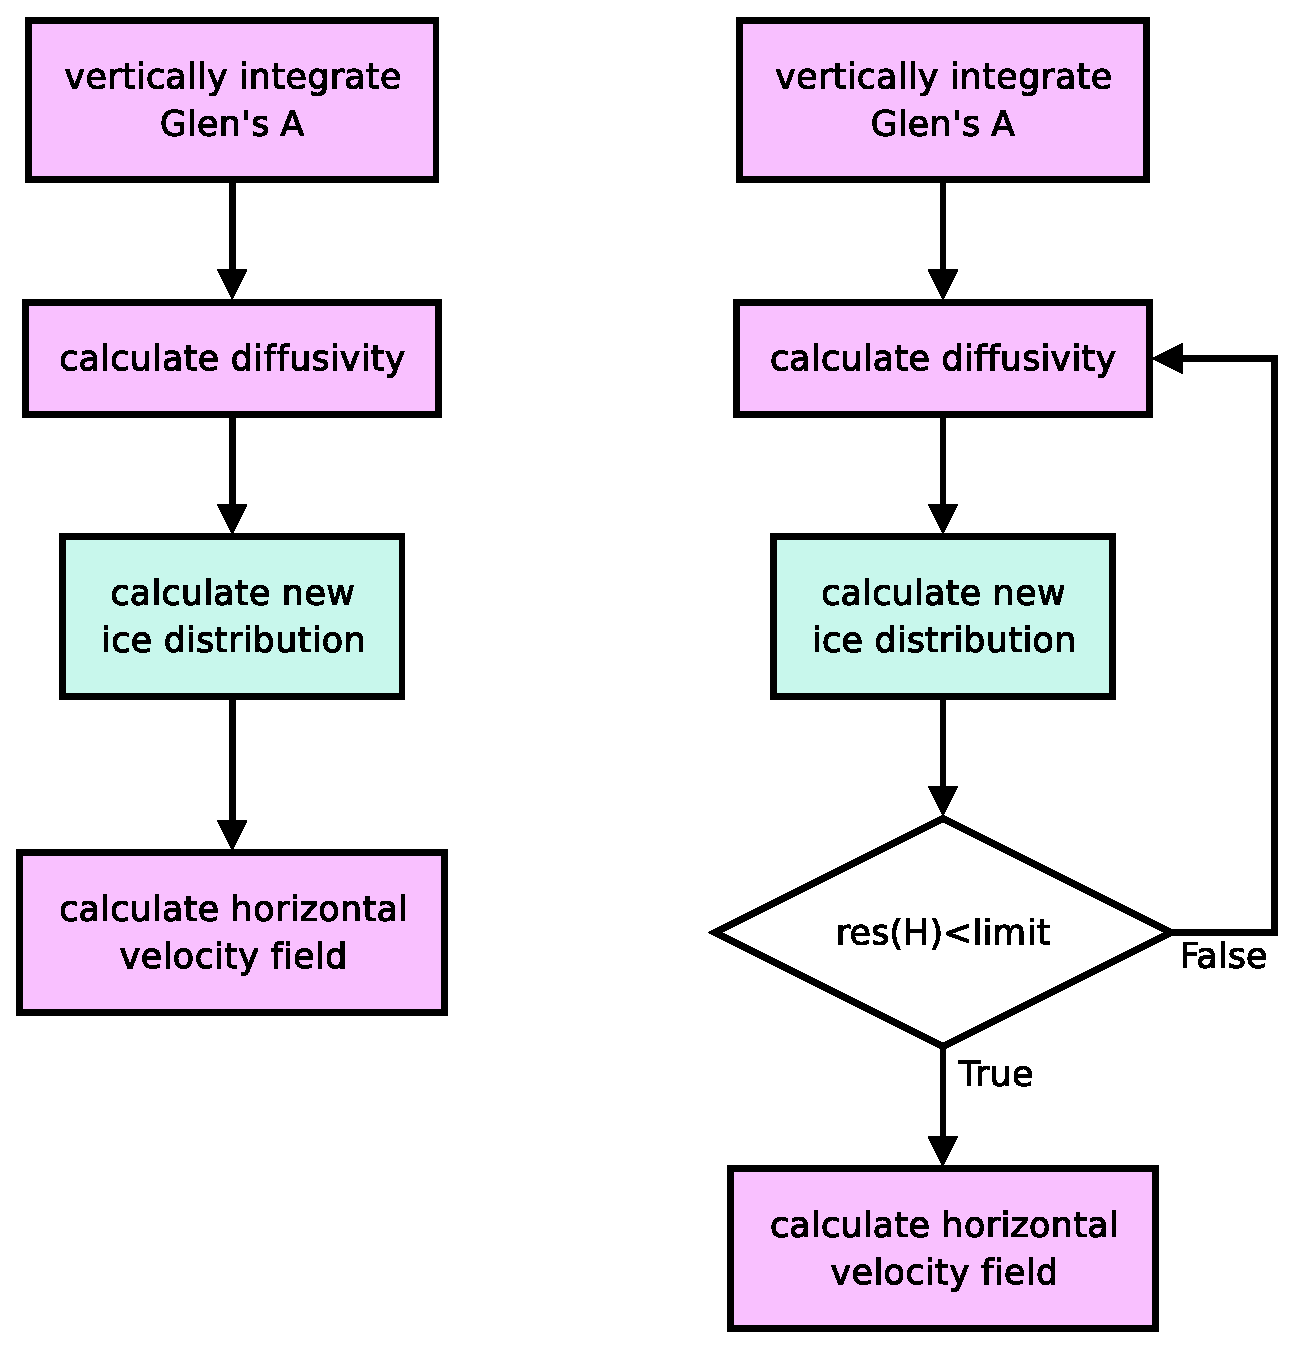
\epsfig{file=\dir/figs/thick_evo.eps,width=0.5\textwidth}
  \caption{Flow diagram showing how the linearised solver (on the left) and the non--linear solver work. The inner, linear iteration is contained within the box labeled ``calculate new ice distribution''.}
  \label{kin.fig.solvers}
\end{figure}

\subsection{Calculating Vertical Velocities}

\subsubsection{Grid Velocity}
The vertical grid moves as a consequence of using a $\sigma$--coordinate system. The grid velocity is
\begin{equation}
  \label{kin.eq.grid_velo}
  w^{\text{grid}}(\sigma)=\frac{\pd s}{\pd t}+\vec u\cdot\vec\nabla s-\sigma\left(\frac{\pd H}{\pd t}+\vec u\cdot\vec\nabla H\right)
\end{equation}
The numerical implementation of Equation \eqref{kin.eq.grid_velo} is straight--forward.

\subsubsection{Vertical Velocity}
The discretised version of the vertical velocity equation \eqref{kin.eq.vert_velo_scaled} is slightly more compilicated because the horizontal velocities are calculated on the $(r,s)$ grid. The vertical velocity at the ice base is $w_{i,j,N}=w^{\text{grid}}_{i,j,N}-b_{i,j}$, where $b_{i,j}$ is the basal melt rate. Integrating from the bottom, the vertical velocity is then
\begin{equation}
  \label{kin.eq.wvel_unc}
  \begin{split}
  w_{i,j,k}=-\sum_{\tilde{k}=N-1}^1\left\{\mathcal{H}_{i,j}\left(\frac{u^x_{i,j,k}+u^x_{i,j,k+1}}{2}+\frac{v^y_{i,j,k}+v^y_{i,j,k+1}}{2}\right)(\sigma_{k+1}-\sigma_k)\right. \\
     +(\tilde{u}_{i,j,k+1}-\tilde{u}_{i,j,k})  \left(\tilde{s}^x_{i,j}-\frac12(\sigma_{k+1}+\sigma_k)\tilde{H}^x_{i,j}\right)  \\
     \left.+(\tilde{v}_{i,j,k+1}-\tilde{v}_{i,j,k})  \left(\tilde{s}^y_{i,j}-\frac12(\sigma_{k+1}+\sigma_k)\tilde{H}^y_{i,j}\right)\right\} + w_{i,j,N}
  \end{split}
\end{equation}
with the weighted ice thickness
\begin{equation*}
  \begin{split}
  \mathcal{H}_{i,j}=\frac{4H_{i,j}+2(H_{i-1,j}+H_{i+1,j}+H_{i,j-1}+H_{i,j+1})}{16}\\
  +\frac{H_{i-1,j-1}+H_{i+1,j-1}+H_{i+1,j+1}+H_{i-1,j+1}}{16}    
  \end{split}
\end{equation*}

This scheme produces vertical velocities at the ice divide which are too small. The vertical velocities on the ice surface are given by the upper kinematic boundary condition, Equation \eqref{kin.eq.upper_bc}. Equation \eqref{kin.eq.wvel_unc} can be corrected with:
\begin{equation}
  \label{kin.eq.wvel_cor}
   w^\ast_{i,j,k}=w_{i,j,k}-(1-\sigma_k)(w_{i,j,k}-{w_s}_{i,j}),
\end{equation}
where ${w_s}_{i,j}$ is the vertical velocity at the ice surface given by \eqref{kin.eq.upper_bc}. Figure \ref{kin.fig.w_profile} shows the different vertical velocities at the ice surface.
\begin{figure}[htbp]
  \centering
  \input{\dir/gnu/w_profile.pslatex}
  \caption{Vertical ice surface velocities of the EISMINT-1 moving margin experiment.}
  \label{kin.fig.w_profile}
\end{figure}
The difference between the vertical velocities calculated by the model and the vertical velocities given by \eqref{kin.eq.upper_bc} at the ice margin are due to the fact that temperatures and velocities are only calculated when the ice is thicker than a certain threshold value which is not met at the ice margin.

Figure \ref{kin.fig.wt_sigma} shows vertical profiles of the vertical velocity at the ice divide and a point half--way between the divide and the domain margin. A corresponding temperature profile is also shown since the vertical velocity determines the vertical temperature advection (see Section \ref{temp.sec.vert_ad}).
\begin{figure}[htbp]
  \centering
  \input{\dir/gnu/wt_sigma.pslatex}
  \caption{Vertical velocity and temperature distribution for columns at the ice divide and a point half--way between the divide and the domain margin.}
  \label{kin.fig.wt_sigma}
\end{figure}
\section{Temperature Solver}
The flow law, Equation \eqref{kin.eq.flowlaw}, depends on the temperature of ice. It is, therefore, necessary to determine how the distribution of ice temperatures changes with a changing ice sheet configuration. The thermal evolution of the ice sheet is described by
\begin{equation}
  \label{temp.eq.temp_z}
  \frac{\pd T}{\pd t}=\frac{k}{\rho c}\nabla^2T-\vec{u}\cdot\vec\nabla T+\frac\Phi{\rho c}-w\frac{\pd T}{\pd z},
\end{equation}
where $T$ is the absolute temperature, $k$ is the thermal conductivity of ice, $c$ is the specific heat capacity and $\Phi$ is the heat generated due to internal friction. In the $\sigma$--coordinate system, Equation \eqref{temp.eq.temp_z}, becomes
\begin{equation}
  \label{temp.eq.temp}
  \frac{\pd T}{\pd t} = \frac{k}{\rho cH^2}\frac{\pd^2T}{\pd\sigma^2} - \vec{u}\cdot\vec\nabla T + \frac{\sigma g}c\frac{\pd \vec{u}}{\pd\sigma}\cdot\vec\nabla s + \frac1H\frac{\pd T}{\pd\sigma}\left(w-w_{\text{grid}}\right)
\end{equation}
The terms represents (1) vertical diffusion, (2) horizontal advection, (3) internal heat generation due to friction and (4) vertical advection and a correction due to the sigma coordinate system. Let's rewrite \eqref{temp.eq.temp} to introduce some names:
\begin{equation}
  \label{temp.eq.temp2}
  \frac{\pd T}{\pd t} = a\frac{\pd^2T}{\pd\sigma^2} +b(\sigma) + \Phi(\sigma) + c(\sigma)\frac{\pd T}{\pd\sigma},
\end{equation}
where
\begin{subequations}
  \begin{align}
    a&=\frac{k}{\rho cH^2} \\
    \label{temp.eq.hadv}
    b(\sigma)&=-\vec{u}\cdot\vec\nabla T\\
    \Phi(\sigma)&=\frac{\sigma g}c\frac{\pd \vec{u}}{\pd\sigma}\cdot\vec\nabla s \\
    c(\sigma)&=\frac1H\left(w-w_{\text{grid}}\right)
  \end{align}
\end{subequations}

\subsection{Vertical Diffusion}
Discretisation of $\pd^2T/\pd\sigma^2$ is slightly complicated because the vertical grid is irregular. Using Taylor series the central difference formulas are
\begin{subequations}
  \begin{align}
    \label{temp.eq.d1}
    \left.\frac{\pd T}{\pd\sigma}\right|_{\sigma_{k-1/2}}&=\frac{T_k-T_{k-1}}{\sigma_k-\sigma_{k-1}}\\
    \intertext{and}
    \label{temp.eq.d2}
    \left.\frac{\pd T}{\pd\sigma}\right|_{\sigma_{k+1/2}}&=\frac{T_{k+1}-T_k}{\sigma_{k+1}-\sigma_k}\\
    \intertext{The second partial derivative is then, also uning central differences:}
    \label{temp.eq.d3}
    \left.\frac{\pd^2 T}{\pd\sigma^2}\right|_{\sigma_k} &= \frac{\left.{\pd T}/{\pd\sigma}\right|_{\sigma_{k+1/2}} - \left.{\pd T}/{\pd\sigma}\right|_{\sigma_{k-1/2}}}{1/2\left(\sigma_{k+1}-\sigma_{k-1}\right)}\\
    \intertext{Inserting \eqref{temp.eq.d1} and \eqref{temp.eq.d2} into \eqref{temp.eq.d3}, we get:}
    \label{temp.eq.d4}
    &=\frac{2(T_{k+1}-T_k)}{(\sigma_{k+1}-\sigma_k)(\sigma_{k+1}-\sigma_{k-1})}-\frac{2(T_k-T_{k-1})}{(\sigma_k-\sigma_{k-1})(\sigma_{k+1}-\sigma_{k-1})}
  \end{align}
\end{subequations}
Finally, the terms of equation \eqref{temp.eq.d4} are rearranged:
\begin{multline}
  \left.\frac{\pd^2 T}{\pd\sigma^2}\right|_{\sigma_k} = \frac{2T_{k-1}}{(\sigma_k-\sigma_{k-1})(\sigma_{k+1}-\sigma_{k-1})} - \frac{2T_k}{(\sigma_{k+1}-\sigma_k)(\sigma_k-\sigma_{k-1})}\\
  + \frac{2T_{k+1}}{(\sigma_{k+1}-\sigma_k)(\sigma_{k+1}-\sigma_{k-1})}
\end{multline}

\subsection{Horizontal Advection}
The horizontal advection term, $- \vec{u}\cdot\vec\nabla T$ is solved using an upwinding scheme. Let's start with the 1--dimensional case. The method discussed can be straightforwadly extented to 2D. As always, the temperature function is expressed as a Taylor series.
\begin{subequations}
  \begin{align}
    \label{temp.eq.taylor1}
    T(x+\Delta x) &=T(x)+\Delta xT'(x)+\frac{\Delta x^2}2T''(x)+\ldots\\
    \intertext{If we subsitute $\Delta x$ with $2\Delta x$, Equation \eqref{temp.eq.taylor1}}
    \label{temp.eq.taylor2}
    T(x+2\Delta x) &=T(x)+2\Delta xT'(x)+2\Delta x^2T''(x)+\ldots
  \end{align}
\end{subequations}
From \eqref{temp.eq.taylor1} and \eqref{temp.eq.taylor2} we can construct a difference formula where the $\mathcal{O}(\Delta x^2)$ error is cancelled, by multiplying \eqref{temp.eq.taylor1} with 4 and substracting the result from \eqref{temp.eq.taylor2}:
\begin{subequations}
  \begin{align}
    \label{temp.eq.forward_h3}
    T_+'(x)&=\frac{4T(x+\Delta x)-T(x+2\Delta x)-3T(x)}{2\Delta x}\\
    \intertext{and similarly for the backward difference:}
    T_-'(x)&=-\frac{4T(x-\Delta x)-T(x-2\Delta x)-3T(x)}{2\Delta x}
    \end{align}
\end{subequations}
So the horizontal advection term in one dimensions becomes:
\begin{equation}
  b_x = -u_x\frac{\pd T}{\pd x}=\frac{-u_x}{2\Delta x}
  \begin{cases}
    -(4T_{i-1}-T_{i-2}-3T_i) & \text{when $u_x>0$} \\
    4T_{i+1}-T_{i+2}-3T_i & \text{when $u_x<0$} \\
  \end{cases}
\end{equation}
A similar expression is found for $b_y$ by simply substituting $y$ for $x$. Finally, the combined horizontal advection term, is simply
\begin{equation}
  b=-\vec{u}\cdot\vec\nabla T=-\left(u_x\frac{\pd T}{\pd x}+u_y\frac{\pd T}{\pd y}\right)=b_x+b_y=b_1+b_2T_i
\end{equation}

\subsection{Heat Generation}
Taking the derivative of \eqref{kin.eq.vert_velo_sigma} with respect to $\sigma$, we get
\begin{equation}
  \frac{\pd u_x}{\pd\sigma} = -2(\rho g)^nH^{n+1}|\vec\nabla s|^{n-1}\frac{\pd s}{\pd x}A(T^\ast)\sigma^n
\end{equation}
Thus,
\begin{equation}
\begin{split}
  \Phi(\sigma) &= \frac{\sigma g}c\frac{\pd \vec{u}}{\pd\sigma}\cdot\vec\nabla s  = \frac{\sigma g}c\left(\frac{\pd u_x}{\pd \sigma}\frac{\pd s}{\pd x} + \frac{\pd u_y}{\pd \sigma}\frac{\pd s}{\pd y}\right)\\
       &= -2(\rho g)^nH^{n+1}|\vec\nabla s|^{n-1}\frac{\sigma g}cA(T^\ast)\sigma^n \left(\left(\frac{\pd s}{\pd x}\right)^2+\left(\frac{\pd s}{\pd y}\right)^2\right) \\
       &= -\frac2{c\rho}(g\sigma\rho)^{n+1}\left(H|\vec\nabla s|\right)^{n+1}A(T^\ast)
\end{split}  
\end{equation}

The constant factor $\frac2{c\rho}(g\sigma\rho)^{n+1}$ is calculated during initialisation in the subroutine \texttt{init\_temp}. This factor is assigned to array \texttt{c1(1:upn)}. \texttt{c1} also includes various scaling factors and the factor $1/16$ to normalise $\mathcal{A}$.

The next factor, $\left(H|\vec\nabla s|\right)^{n+1}$ is calculated in the subroutine \texttt{finddisp}:
\begin{equation}
  {c_2}_{i,j} = \left(\tilde{H}_{i,j}\sqrt{\tilde{S_x}_{i,j}^2+\tilde{S_y}_{i,j}^2}\right)^{n+1},
\end{equation}


The final factor is found by averaging over the neighbouring nodes:
\begin{equation}
  \mathcal{A}_{i,j}=4A_{i,j}+2(A_{i-1,j}+A_{i+1,j}+A_{i,j-1}+A_{i,j+1})+(A_{i-1,j-1}+A_{i+1,j-1}+A_{i+1,j+1}+A_{i-1,j+1})
\end{equation}

\subsection{Vertical Advection}
The vertical advection term, $\pd T/\pd\sigma$ is solved using the central difference formula for unevenly spaced nodes:
\begin{equation}
  \frac{\pd T}{\pd\sigma}=\frac{T_{k+1}-T_{k-1}}{\sigma_{k+1}-\sigma_{k-1}}
\end{equation}

\subsection{Boundary Conditions}
At the upper boundary, ice temperatures are set to the surface temperature, $T_{\text{surf}}$. At the ice base, the boundary condition depends on whether the base is melting or not:
\begin{subequations}
  \begin{align}
    T(1) &= T_{\text{pmp}} \quad\text{if $T(1)\ge T_{\text{pmp}}$}\\
    \left.\frac{\pd T}{\pd\sigma}\right|_{\sigma=1}&=-\frac{GH}k \quad\text{if $T(1)<T_{\text{pmp}}$}\\
    \intertext{If the ice is floating, basal temperatures are kept constant, i.e. }
    \frac{\pd T(1)}{\pd t} & = 0
  \end{align}
\end{subequations}
When the ice is floating, basal temperatures are hold constant.

\subsection{Putting it all together}
Equation \eqref{temp.eq.temp} is solved for each ice column. The horizontal dependency of the horizontal advection term, \eqref{temp.eq.hadv}, is resolved by iterating the vertical solution. Putting the individual terms together using a fully explicit finite differences scheme, Equation \eqref{temp.eq.temp2} becomes
\begin{subequations}
  \begin{multline}
    \label{temp.eq.temp3a}
    \frac{T_{k,t+1}-T_{k,t}}{\Delta t} = \left(\frac{2aT_{k-1,t}}{(\sigma_k-\sigma_{k-1})(\sigma_{k+1}-\sigma_{k-1})} - \frac{2aT_{k,t}}{(\sigma_{k+1}-\sigma_k)(\sigma_k-\sigma_{k-1,t})}\right. \\
    \left.+ \frac{2aT_{k+1,t}}{(\sigma_{k+1}-\sigma_k)(\sigma_{k+1}-\sigma_{k-1})}\right)+{b_1}_{k,t}+{b_2}_kT_{k,t}+\Phi_k+c_k\frac{T_{k+1,t}-T_{k-1,t}}{\sigma_{k+1}-\sigma_{k-1}}
\end{multline}
and similarly the fully implicit scheme
  \begin{multline}
    \label{temp.eq.temp3b}
    \frac{T_{k,t+1}-T_{k,t}}{\Delta t} = \left(\frac{2aT_{k-1,t+1}}{(\sigma_k-\sigma_{k-1})(\sigma_{k+1}-\sigma_{k-1})} - \frac{2aT_{k,t+1}}{(\sigma_{k+1}-\sigma_k)(\sigma_k-\sigma_{k-1,t+1})}\right. \\
    \left.+ \frac{2aT_{k+1,t+1}}{(\sigma_{k+1}-\sigma_k)(\sigma_{k+1}-\sigma_{k-1})}\right)+{b_1}_{k,t+1}+{b_2}_kT_{k,t+1}+\Phi_k+c_k\frac{T_{k+1,t+1}-T_{k-1,t+1}}{\sigma_{k+1}-\sigma_{k-1}}
\end{multline}
\end{subequations}
Taking the average of Equations \eqref{temp.eq.temp3a} and \eqref{temp.eq.temp3b} gives the \emph{Crank--Nicholson scheme}. The resulting equation is then rearranged and terms of $T_{k-1,t+1}$, $T_{k,t+1}$ and $T_{k+1,t+1}$ are combined to give the tri--diagonal system
\begin{equation}
  \alpha_kT_{k-1,t+1}+\beta_kT_{k,t+1}+\gamma_kT_{k+1,t+1}=\delta_k
\end{equation}
where, for $k=2,N-1$
\begin{subequations}
  \begin{align}
    \alpha_k &= -\frac12\frac{2a\Delta t}{(\sigma_k-\sigma_{k-1})(\sigma_{k+1}-\sigma_{k-1})}+\frac12\frac{c_k\Delta t}{\sigma_{k+1}-\sigma_{k-1}} \\
    \beta_k &= 1+\frac12\frac{2a\Delta t}{(\sigma_{k+1}-\sigma_k)(\sigma_k-\sigma_{k-1})}-\frac12{b_2}_k\Delta t=1-\alpha_k-\gamma_k-\frac12{b_2}_k\Delta t\\
    \gamma_k &= -\frac12\frac{2a\Delta t}{(\sigma_{k+1}-\sigma_k)(\sigma_{k+1}-\sigma_{k-1})}-\frac12\frac{c_k\Delta t}{\sigma_{k+1}-\sigma_{k-1}} \\
    \delta_k &= -\alpha_kT_{k-1,t}+(2-\beta_k)T_{k,t}-\gamma_kT_{k+1,t}+\frac12({b_1}_{k,t}+{b_1}_{k,t+1})\Delta t+\Phi_k\Delta t
  \end{align}

\subsubsection{Boundary Conditions}
At the upper boundary:
\begin{equation}
  \alpha_1=0,\quad\beta_1=1,\quad\gamma_1=0,\quad\delta_1=T_{\text{surf}}
\end{equation}
\end{subequations}


The lower boundary condition is somewhat more complicated. Here we only look at the case when the temperature is below the pressure melting point of ice. BC for floating ice and temperatures at the pressure melting point of ice are trivial. The geothermal heat flux is applied at the lower boundary, i.e. Equation \eqref{temp.eq.d2} becomes
\begin{equation}
  \label{temp.eq.d2-lb}
  \left.\frac{\pd T}{\pd\sigma}\right|_{\sigma_{k+1/2}}=-\frac{GH}k
\end{equation}
Assuming that $\sigma_k-\sigma_{k-1}=\sigma_{k+1}-\sigma_k=\Delta\sigma$ and inserting \eqref{temp.eq.d1} and \eqref{temp.eq.d2-lb} into \eqref{temp.eq.d3}, the second partial derivative becomes
\begin{equation}
  \left.\frac{\pd^2 T}{\pd\sigma^2}\right|_{\sigma_N} = \left(-\frac{GH}k-\frac{T_N-T_{N-1}}{\Delta\sigma}\right)/\Delta\sigma=-\frac{GH}{k\Delta\sigma}-\frac{T_N-T_{N-1}}{\Delta\sigma^2}
\end{equation}
Inserting the new conduction term and replacing the derivative of the vertical advection term with the Neuman boundary condition, Equation \eqref{temp.eq.temp3a} becomes
\begin{subequations}
  \begin{equation}
    \frac{T_{N,t+1}-T_{N,t}}{\Delta t} = -a\left(\frac{GH}{k\Delta\sigma}+\frac{T_{N,t}-T_{N-1,t}}{\Delta\sigma^2}\right)+{b_1}_{N,t}+{b_2}_NT_{N,t}+\Phi_N-c_N\frac{GH}k
  \end{equation}
  and similarly for Equation \eqref{temp.eq.temp3b}
  \begin{multline}
    \frac{T_{N,t+1}-T_{N,t}}{\Delta t} = -a\left(\frac{GH}{k\Delta\sigma}+\frac{T_{N,t+1}-T_{N-1,t+1}}{\Delta\sigma^2}\right)+{b_1}_{N,t+1}+{b_2}_NT_{N,t+1}\\
    +\Phi_N-c_N\frac{GH}k
  \end{multline}
\end{subequations}
The elements of the tri--diagonal system at the lower boundary are then
\begin{subequations}
  \begin{gather}
    \alpha_N =-\frac{a\Delta t}{2(\sigma_N-\sigma_{N-1})^2}\\
    \beta_N = 1-\alpha_N+\frac12{b_2}_N\Delta t\\
    \gamma_N = 0 \\
    \begin{split}
      \delta_N =&-\alpha_NT_{N-1,t}+(2-\beta_N)T_{N,t}-a\frac{GH\Delta t}{k(\sigma_N-\sigma_{N-1})}\\
      &+\frac12({b_1}_{N,t}+{b_1}_{N,t+1})\Delta t+\Phi_N\Delta t-c_N\frac{GH\Delta t}k
    \end{split}
  \end{gather}
\end{subequations}


\section{Isostatic Adjustment}
The ice sheet model includes simple approximations for calculating isostatic adjustment. These approximations depend on how the lithosphere and the mantle are treated. For each subsystem there are two models. The lithosphere can be described as a
\begin{description}
\item[\textbf{local lithosphere:}] the flexural rigidity of the lithosphere is ignored, i.e. this is equivalent to ice floating directly on the asthenosphere;
\item[\textbf{elastic lithosphere:}] the flexural rigidity is taken into account;
\end{description}
while the man is treated as a
\begin{description}
\item [\textbf{fluid mantle:}] the mantle behaves like a non-viscous fluid, isostatic equilibrium is reached instantaneously;
\item [\textbf{relaxing mantle}] the flow within the mantle is approximated by an exponentially decaying hydrostatic response function, i.e. the mantle is treated as a viscous half space.
\end{description}
See my PhD thesis for implementation details.

\chapter{Developer Guide}
\renewcommand{\dir}{dg}
\section{Introduction}

The `design' of GLIMMER is a consequence of the way it has been
developed. Initially, as a stand-alone model with a single domain, module
variables were used to hold all model fields and parameters. With the move to
use GLIMMER as the ice model component within GENIE, and the desire to enable
several active regions to be run simultaneously, the module variables were
converted into components of derived types, and an extra layer added on top of
the exisiting structure to deal with global fields and parameters, and deal
with the downscaling/interpolation of input fields. The result is a structure
that is probably more complex than it needs to be, but still hopefully
reasonably logical.


\section{Physics documentation}

\subsection{Ice temperature evolution routines}

\subsubsection{Summary}
Call structure (filenames in brackets).
\begin{itemize}
    \item subroutine testinisthk [glimmer\_setup] and
    \item subroutine glimmer\_i\_tstep [glimmer\_object] call
    \item subroutine timeevoltemp [glimmer\_temp] calls
    \item subroutine calcartm [glimmer\_temp] and
    \item subroutine timeders [glimmer\_thck] and
    \item subroutine gridwvel [glimmer\_velo] and
    \item subroutine wvelintg [glimmer\_velo] and
    \item subroutine chckwvel [glimmer\_velo] and
    \item subroutine finddisp [glimmer\_temp] and
    \item subroutine hadvall [glimmer\_temp] and
    \item subroutine hadvpnt [glimmer\_temp] and
    \item subroutine findvtri [glimmer\_temp] and
    \item subroutine tridag [glimmer\_temp] and
    \item subroutine corrpmpt [glimmer\_temp] and
    \item subroutine swapbndt [glimmer\_temp] and
    \item subroutine calcbmlt [glimmer\_temp] and
    \item subroutine calcflwa [glimmer\_temp]
\end{itemize}

\noindent Modules used.
\begin{itemize}
    \item
\end{itemize}

\subsubsection{Introduction}
The section describes the routines that are concerned with
calculating the three-dimensional distribution of temperature
within the ice mass.  They can be broken down into five groups.
\begin{itemize}
    \item determining air temperature (upper boundary
    condition) [\texttt{calcartm}];
    \item determining vertical velocity field from existing
    horizontal velocity fields (normally only needed if temperature is being calculated) [\texttt{wvelintg}, chckwvel];
    \item routines associated with vertical grid coordinate
    system [\texttt{gridwvel}, \texttt{timeders}];
    \item the main temperature solver [\texttt{finddisp, hadvall, hadvpnt, findvtri, tridag, corrpmpt, swapbndt}];
    \item ancillary calculations that only make sense if temperature is being calculated
    [\texttt{calcbmlt}, \texttt{calcflwa}].
\end{itemize}

The basic quantity returned is a three-dimensional grid of
temperature in $\circ^{-1}$C (uncorrected for variations in
pressure melting point and unscaled).  Temperature is held in the
array \texttt{temp} and will be referred to here using the symbol
$T$.

In addition to temperature a number of other quantities are
calculated by these routines.  They include: basal melt rate ($m$
\texttt{bmlt} m yr$^{-1}$ scaled using \texttt{thk0/tim0}); basal
water depth ($W$ \texttt{bwat} m scaled using \texttt{thk0});
vertical velocity ($w$ \texttt{wvel} m yr$^{-1}$ scaled using
\texttt{thk0/tim0}); vertical velocity of numerical grid ($w_0$
\texttt{wgrd} m yr$^{-1}$ scaled using \texttt{thk0/tim0}); Glen's
A ($A$ \texttt{flwa} Pa$^{-3}$ yr$^{-1}$ scaled using
\texttt{vis0}); air temperature ($T_a$ $\circ^{-1}$C unscaled).
All scales are held in the module \texttt{paramets} in
\textbf{\texttt{glimmer\_paramets}}.

Three options are currently available for calculating $T$. The
particular option chosen is controlled by the input parameter
\texttt{whichtemp} (\texttt{gln} file).

\begin{description}
    \item[0] Set whole column to the appropriate surface air temperature ($T_a$).
    \item[1] This option is the main solver that determines temperature
    at the new time step from the appropriate three-dimensional
    advection-diffusion equation.
    \item[2] Set the upper surface temperature to $T_a$ and do a linear
    interpolation from this value to 0 $^\circ$C at the lower
    surface. Check for pressure melting and adjust any
    temperatures that are above melting point.
\end{description}

The subroutine \texttt{timeevoltemp} controls calculation of the
$T$ etc. It is called in the main time loop in
\textbf{\texttt{glimmer\_object}} and resides in
\textbf{\texttt{glimmer\_temp}}.

\subsection{Mass balance routines}

\subsubsection{Summary}
Call structure (filenames in brackets).
\begin{itemize}
    \item subroutine testinisthk [glimmer\_setup] and
    \item subroutine glimmer\_i\_tstep [glimmer\_object] call
    \item subroutine calcacab [glimmer\_thck] calls
    \item subroutine masbgrn [glimmer\_degd]
\end{itemize}

\noindent Modules used.
\begin{itemize}
    \item glimmer\_degd [glimmer\_degd]
    \item paramets [glimmer\_paramets]
\end{itemize}

\subsubsection{Introduction} The model contains a variety of surface
mass balances schemes. The basic quantity returned is a
two-dimensional grid of surface mass balance in m yr$^{-1}$ ice
equivalents (positive for net annual accumulation and negative for
net annual ablation) scaled using the quantity \texttt{acc0} (see
module \texttt{paramets} in \textbf{\texttt{glimmer\_paramets}}).
The particular option chosen is controlled by the input parameter
\texttt{whichacab} (\texttt{gln} file).

Surface mass balance is held in the array \texttt{acab} and will
be referred to here using the symbol $b$. Three options are
currently available for calculating $b$.

\begin{description}
    \item[0] Set up radial mass balance field.  This option is
    primarily for EISMINT moving-margin benchmarks.  It uses the input
    parameter \texttt{nmsb(1:3)} (\texttt{gln} file).
    \item[1] This option is appropriate for Greenland calculations
    and does a day-degree calculation for mass balance.
    \item[2] Simply sets the mass balance equal to the
    precipitation field.  This option is suitable for modelling
    Antarctica or the EISMINT fixed-margin benchmark.
\end{description}

It is hoped (July 2004) to add a surface energy-balance option (3)
this year.

The subroutine \texttt{calcacab} controls calculation of the $b$.
It is called in the main time loop in
\textbf{\texttt{glimmer\_object}} and resides in
\textbf{\texttt{glimmer\_thck}}.

\subsubsection{EISMINT code (option 0)}
A radial mass balance is created which is centred on the middle of
the model grid
\begin{equation}\label{eismintb}
    b(x,y) = \min(b_1,b_2\times(b_3-d))
\end{equation}
where $d$ is the distance in m from the middle of the grid and
$b_1$ is in m yr$^{-1}$, $b_2$ is in yr$^{-1}$ and $b_3$ is in m
(all have been scaled by the time they reach this subroutine).
Details of the EISMINT moving-margin test can be found in
\emph{Huybrechts and others} [1996] and the values for the $b$
parameters are: 0.5 m yr$^{-1}$, 10$^{-5}$ yr$^{-1}$ and 4.5
$\times 10^5$ m.

\paragraph{References}

Huybrechts and others (1996) The EISMINT benchmarks for testing
ice-sheet models, \emph{Annals of Glaciology} \textbf{23}, 1-12.

\subsubsection{Greenland code (option 1)}
This is the most complicated option to date.  It calls subroutine
\texttt{masbgrn}, which resides in
\textbf{\texttt{glimmer\_degd}}.

This option follows the EISMINT Greenland parameterization.  It
contains two basic components.  The first is a day-degree
calculation of ablation, and the second is an estimation of
refreezing.

Inputs are: mean annual air temperature (\texttt{artm}); annual
air temperature half range (\texttt{arng}); precipitation
(\texttt{prcp}); and latitude (\texttt{lati}).  All on
two-dimensional, spatial grids. Temperatures and latitude are not
scaled, while precipitation is assumed to have already been
scaled.  Latitude is only used as a mask and calculation are
performed only if it is non-zero (may need to look at this).

In addition to outputting \texttt{acab}, the routines output the
calculated ablation \texttt{ablt} (also scaled).  Note that any
corrections (for instance to account for changing altitude, air
temperature and atmospheric moisture) to the precipitation field
are delt with elsewhere (see \texttt{\textbf{glimmer\_mbal}}).

\paragraph{Day-degree calculation}
The parameters used in these calculations are set in
\texttt{glimmer\_pddcalc} in \textbf{\texttt{glimmer\_modu}}.

The fairly large amount of computation required here means that a
look-up table approach has been implemented.  If this is the first
time that the subroutine has been used then the look-up table is
constructed in subroutine \texttt{pddtabgrn}.

The table has two dimensions: mean annual air temperature ($T_a$)
(as the second index) and annual air temperature half range (i.e.,
from July's mean to the annual mean $\Delta T_a$) (as the first
index).  Following \emph{Huybrechts and others} [1991], daily air
temperatures ($T_a^\prime$) are assumed to follow a sinusoidal
cycle
\begin{equation}
    T_a^\prime = T_a + \Delta T_a \cos \left( \frac{2 \pi t}{A}
    \right) + \textbf{R}(0,\sigma)
\end{equation}
where $A$ is the period of a year and $R$ is a random fluctuation
drawn from a normal distribution with mean 0 $^\circ$C and
standard deviation $\sigma$ $^\circ$C. \emph{Huybrechts and
others} [1991] indicate that the number of positive degree days
(D, $^\circ$C days) for this temperature series can be evaluated
as
\begin{equation}\label{pdd}
    D = \frac{1}{\sigma \sqrt{2 \pi}}
    \int\limits_0^A
    \int\limits_0^{T_a^\prime+2.5\sigma}
    T_a \times \exp \left( \frac{-(T_a-T_a^\prime)^2}{2 \sigma^2} \right) dT
    dt
\end{equation}
where $t$ is time.  The table is completed by evaluating this integral using a
public-domain algorithm (Romberg integration), by {\it Bauer} [1961]. The
inner and outer integrals are coded as two subroutines
(\texttt{inner\_integral} and \texttt{pdd\_integrand}), which call the Romburg
integration recursively.

The main parameter needed is the assumed standard deviation of
daily air temperatures, which is set in
\textbf{\texttt{glimmer\_pddcalc}} (typically 5 $^\circ $C).  The
module also contains information on the size and extent (in terms
of $T_a$ and $\Delta T_a$) of the table to be constructed.

The table has now been constructed and we can enter the main loop
in \texttt{masbgrn}, which visits each cell in the numerical grid
in turn. Note that the variable \texttt{lati} is used as a mask
and calculation are made only for non-zero values of \texttt{lati}
(both \texttt{ablt} and \texttt{acab} are otherwise set to zero).

The positive-degree days are then looked up in the table just
described (as a function of $T_a$ and $\Delta T_a$). We take care
to check that this look up is in done within the bounds of the
table.  The final value of $P$ is determined using bi-linear
interpolation given the four nearest entries in the table to the
actual values of $T_a$ and $\Delta T_a$.

The remainder of the loop completes the calculation of the
ablation and accumulation given this value for $P$.

\paragraph{Mass balance calculation} The parameters used in these
calculations are set in \texttt{paramets} in
\textbf{\texttt{glimmer\_paramets}}. Note, in particular, the
day-degree factors have been converted from ice to water
equivalents using the ratio of densities.  They are also scaled.

We use the following symbols: $a$ is total annual ablation; $a_s$
is potential snow ablation; $b_0$ is the capacity of the snowpack
to hold meltwater by refreezing; the total number of positive
degree days ($D$); day-degree factors for snow and ice ($f_s$ and
$f_i$); and the fraction of snowfall that can be held in the
snowpack as refrozen meltwater ($W_max$).

 First,
determine the depth of superimposed ice ($b_0$) that would have to
be formed before runoff (mass loss) occurs as a constant fraction
($W_{max}$) of precipitation ($P$)
\begin{equation}
    b_0=W_{max} P.
\end{equation}
Now determine the amount of snow melt by applying a constant
day-degree factor for snow to the number of positive day-degrees
\begin{equation}
    a_s=f_s D.
\end{equation}
We now compare the potential amount of snow ablation with the
ability of the snow layer to absorb the melt.  Three cases are
possible. First, all snow melt is held within the snowpack and no
runoff occurs ($a=0$).  Second, the ability of the snowpack to
hold meltwater is exceeded but the potential snow ablation is
still less than the total amount of precipitation so that
$a=a_s-b_0$. Finally, the potential snow melt is greater than the
precipitation (amount of snow available), so that ice melt ($a_i$)
has to be considered as well.  The total ablation is therefore the
sum of snow melt (total precipitation minus meltwater held in
refreezing) and ice melt (deduct from total number of degree days,
the number of degree days needed to melt all snowfall and convert
to ice melt)
\begin{equation}
    a=a_s + a_i = P - b_0 + f_i \left( D-\frac{P}{f_s} \right).
\end{equation}
We now have a total annual ablation, and can find total net mass
balance as the difference between the total annual precipitation
and the total annual ablation.

Note that this methodology is fairly standard and stems from a
series of Greenland papers by Huybrechts, Letreguilly and Reeh in
the early 1990s.

\paragraph{References}

Bauer (1961) \emph{Comm. ACM} \textbf{4}, 255.

Huybrechts, Letreguilly and Reeh (1991) \emph{Palaeogeography,
Palaeoclimatology, Palaeoecology (Global and Planetary Change)}
\textbf{89}, 399-412.

Letreguilly, Reeh and  Huybrechts (1991) \emph{Palaeogeography,
Palaeoclimatology, Palaeoecology (Global and Planetary Change)}
\textbf{90}, 385-394.

Letreguilly, Huybrechts  and  Reeh (1991) \emph{Journal of
Glaciology} \textbf{37}, 149-157.

\subsubsection{Antarctic code (option 2)}
This option simply sets $b$ to the array \texttt{prcp}.

\subsubsection{Issues}
\begin{enumerate}
    \item Use of \texttt{lati} as a mask seems unnecessary perhaps
    use land/sea mask.
    \item Need to discuss location of precipitation calculations
    and where they are called from.
    \item Ditto for air temperature calculations.
\end{enumerate}


\section{Data structure}

The derived type \texttt{glimmer\_params} is the top-level data-structure in
GLIMMER. It contains the global parameters for the model, as well as the
global fields used in the temporal averaging of input fields. Its primary
function, however, is to hold an array of ice model instances (type
\texttt{glimmer\_instance}). This array is allocated at run-time. Each ice
model instance contains instances of derived types (\texttt{projection} and
\texttt{downscale}) concerning the relationship between the local and global
model grids, as well as upscaling parameters (which should have their own
derived type, really), and an instance of \texttt{glimmer\_global\_type}. This
last derived type contains single instances of eighteen other derived types,
which were replacements for the variable-containing modules of the original
ice model. It is debatable whether \texttt{glimmer\_global\_type} is strictly necessary,
and it might be worth reorganising the whole structure at some point, though
this would obviously be a big job. The situation is summarised in figure
\ref{main_class_diagram}.

\begin{figure}
\centering
\epsfig{figure=\dir/figures/class_diagram.eps,width=\textwidth}
\caption{Main `Class Diagram' for GLIMMER. The relationship between the top-level
  \texttt{glimmer\_params} type and its component types is shown. The
  components of the \texttt{glimmer\_global\_type} type are formed from the
  modules of the original ice model.}
\label{main_class_diagram}
\end{figure}

\section{Configuration File Parser}\label{dg.sec.config_file}
The run--time behaviour of the ice sheet model is controlled by configuration files. The old file format is based on Fortran namelists. The new configuration file format is loosely based on the format of Windows \texttt{.ini} files with sections containing name/value pairs. The new format is more flexible and can be easily understood by reading the configuration files. This section contains a description of the configuration file parser API.

\subsection{File Format}
The parser assumes a maximum number of 250 characters per line. Leading and trailing white space is ignored. Names are case sensitive.
\begin{description}
\item[Comments:] Empty lines and lines starting with \texttt{!}, \texttt{;} or \texttt{\#} are ignored.
\item[Sections:] Section names are enclosed with square prackets, \texttt{[]} and can be 20 character long.
\item[Parameters:] Parameter names are separated from their associated values with either \texttt{:} or \texttt{=}. The names can be 20 characters long. Values can be 200 characters long.
\end{description}

An example configuration file:
\begin{verbatim}
;a comment
[a section]
an_int  : 1
a_float = 2.0
a_char  = hey, this is rather cool
an_array = 10. 20. -10. 40. 100.

[another section]
! more comments
foo : bar
\end{verbatim}

\subsection{Architecture Overview}
The configuration data is stored as linked list. Each section is described by the following list element:
\begin{verbatim}
  type ConfigSection
     character(len=namelen) :: name
     type(ConfigValue), pointer :: values=>NULL()
     type(ConfigSection), pointer :: next=>NULL()
  end type ConfigSection
\end{verbatim}
The parameter name/value pairs defined in each section are stored in another linked list:
\begin{verbatim}
  type ConfigValue
     character(len=namelen) :: name
     character(len=valuelen) :: value
     type(ConfigValue), pointer :: next=>NULL()
  end type ConfigValue
\end{verbatim}
These linked lists are setup and read using subroutines.

\subsection{API}
\begin{description}
\item[Reading configuration files] Configuration files are read using \texttt{ConfigRead}. This subroutine parses the configuration file and populates the linked lists.
\begin{verbatim}
subroutine ConfigRead(fname,config)
  character(len=*), intent(in) :: fname
  type(ConfigSection), pointer :: config
end subroutine ConfigRead
\end{verbatim}
The pointer \texttt{config} contains the first section of the configuration file.
\item[Dumping configuration] The subroutine \texttt{PrintConfig} traverses the linked lists and prints them to standard output.
\begin{verbatim}
subroutine PrintConfig(config)
  type(ConfigSection), pointer :: config
end subroutine PrintConfig(config)
\end{verbatim}
\item[Searching for a Section] The subroutine \texttt{GetSection} can be used to find a specific section.
\begin{verbatim}
subroutine GetSection(config,found,name)
  type(ConfigSection), pointer :: config
  type(ConfigSection), pointer :: found
  character(len=*),intent(in) :: name
end subroutine GetSection
\end{verbatim}
On exit the pointer \texttt{found} will point to the first section called \texttt{name}. \texttt{found} points to \texttt{NULL()} if the section \texttt{name} is not found.
\item[Reading parameters] Paramter name/value pairs are found using the \texttt{GetValue} family of subroutines. \texttt{GetValue} provides an interface to the individual subroutines \texttt{GetValueChar}, \texttt{GetValueInt}, \texttt{GetValueReal}, \texttt{GetValueIntArray} and \texttt{GetValueRealArray}.
\begin{verbatim}
subroutine GetValue(section,name,val)
  type(ConfigSection), pointer :: section
  character(len=*),intent(in) :: name
  sometype :: val
  integer,intent(in), optional :: numval
end subroutine GetValue
\end{verbatim}
\texttt{section} is the section that should be searched for the parameter \texttt{name}. On exit \texttt{val} contains the parameter value if it is found, otherwise it is unchanged. 

The array versions of \texttt{GetValue} expect value to be a pointer to a one--dimensional array. \texttt{val} is deallocated if it was allocated on entry. The array versions of \texttt{GetValue} also accept an optional value, \texttt{numval}, with which the maximum number of array elements can be set. The default is 100. Array elements are separated by white space.
\end{description}

\section{netCDF I/O}
The netCDF\footnote{\texttt{http://www.unidata.ucar.edu/packages/netcdf/}} library is used for platform independent, binary file I/O. GLIMMER makes use of the f90 netCDF interface. The majority of the source files are automatically generated from template files and a variable definition file using a python script.

Basic netCDF I/O works. The netCDF subsystem uses the configuration file API, described in Section \ref{dg.sec.config_file}. The two major missing aspects are CF\footnote{\texttt{http://www.cgd.ucar.edu/cms/eaton/cf-metadata/index.html}} compliance and storing parameters defining the geographic projection used.

\subsection{Data Structures}
Dimension and variable IDs are stored in the derived type \texttt{glimmer\_nc\_stat}. The ID of a particular netCDF variable can be found by using the corresponding index (variable name prefixed with \texttt{NC\_B\_}, e.g. the index of the ice thickness variable, \texttt{thk}, is \texttt{NC\_B\_THK} and the variable ID is then \texttt{varids(NC\_B\_THK)}. Meta data (such as title, institution and comments) is stored in the derived type \texttt{glimmer\_nc\_meta}.

Input and output files are managed by two separate linked lists. Elements of the input file list contain the number of available time slices and information describing which time slice(s) should be read. Output file elements describe how often data should be written and the current time.

\subsection{The Code Generator}
Much of the code needed to do netCDF I/O is very repetative and can therefore be automatically generated. The code generator, \texttt{generate\_ncvars.py}, is written in python and produces source files from a templeate \texttt{.in} and the variable definition file, see Section \ref{dg.sec.vdf}. The templates are valid source files, all the generator does is replace special comments with the code generated from the variable file. Each supported template file is handled by a separate class derived from a base class. For further information check the documentation of \texttt{generate\_ncvars.py}\footnote{run \texttt{pydoc generate\_ncvars.py}}.

\subsection{Variable Definition File}\label{dg.sec.vdf}
All netCDF variables are defined in a control file, \texttt{ncdf\_vars.def}. Variables can be modified/added by editing this file. The file is read using the python \texttt{ConfigParser} module. The format of the file is similar to Windows \texttt{.ini} files, lines beginning with \texttt{\#} or \texttt{;} or empty lines are ignored. A new variable definition block starts with the variable name in square brackets []. Variables are further specified by parameter name/value pairs which are separated by \texttt{:} or \texttt{=}. Parameter names and their meanings are summarised in Table \ref{dg.tab.vdf}. All parameter names not recognised by the code generator (i.e. not in Table \ref{dg.tab.vdf}) are added as variable attributes.

\begin{table}[htbp]
 \begin{center}
  \begin{tabular}{|l|p{10cm}|}
    \hline
    name & description \\
    \hline
    \hline
    \texttt{dimensions} & List of comma separated dimension names of the variable. C notation is used here, i.e. the slowest varying dimension is listed first.\\
    \hline
    \texttt{data} & The variable to be stored/loaded. The f90 variable is assumed to have one dimension smaller than the netCDF variable, i.e. f90 variables are always snapshots of the present state of the model. Variables which do not depend on time are not handled automatically. Typically, these variables are filled when the netCDF file is created.\\
    \hline
    \texttt{factor} & Variables are multiplied with this factor on output and divided by this factor on input. Default: 1.\\
    \hline
    \texttt{load} & Set to 1 if the variable can be loaded from file. Default: 0.\\
    \hline
    \texttt{units} & UDUNITS compatible unit string describing the variable units.\\
    \hline
    \texttt{long\_name} & A more descriptive name of the variable.\\
    \hline
    \texttt{standard\_name} & The corresponding standard name defined by the CF standard.\\
    \hline
  \end{tabular}
  \caption{List of accepted variable definition parameters.}
  \label{dg.tab.vdf}
 \end{center}
\end{table}



\appendix
\renewcommand{\dir}{ug}
\chapter{netCDF Variables}
%%%%%%%%%%%%%%%%%%%%%%%%%%%%%%%%%%%%%%%%%%%%%%%%%%%%%%%%%%%%%%%%%%%%%%%%%%%%%%%%
% WARNING: this file was automatically generated on
% Tue, 11 Jan 2005 15:56:57 +0000
% from varlist.tex.in
%%%%%%%%%%%%%%%%%%%%%%%%%%%%%%%%%%%%%%%%%%%%%%%%%%%%%%%%%%%%%%%%%%%%%%%%%%%%%%%%

\label{ug.sec.varlist}
The following list shows all the variable names used by GLIMMER. Only variables marked with $^\ast$ are loaded by the input routines. Append \texttt{\_spot} to the variable name to get single location version of the variable.
\begin{center}
    \tablefirsthead{%
    \hline
        Name&  Description & Units\\
    \hline
    \hline}
  \tablehead{%
    \hline
    \multicolumn{3}{|p{0.98\textwidth}|}{\emph{\small continued from previous page}}\\
    \hline
        Name&  Description & Units\\
    \hline
    \hline}
  \tabletail{%
    \hline
    \multicolumn{3}{|r|}{\emph{\small continued on next page}}\\
    \hline}
  \tablelasttail{\hline}
  \begin{supertabular}{|l|p{8cm}|c|}
    \hline
\texttt{ablt} & ablation & meter/year\\
\hline
\texttt{acab} & accumulation, ablation rate & meter/year\\
&CF name: \texttt{land\_ice\_surface\_mass\_balance}&\\
\hline
\texttt{arng} & annual temperature range & degree\_Celcius\\
\hline
\texttt{artm} & annual mean air temperature & degree\_Celcius\\
&CF name: \texttt{surface\_temperature}&\\
\hline
\texttt{bmlt} & basal melt rate & meter/year\\
&CF name: \texttt{land\_ice\_basal\_melt\_rate}&\\
\hline
\texttt{btemp} & basal ice temperature & degree\_Celcius\\
\hline
\texttt{btrc} & basal slip coefficient & meter/pascal/year\\
\hline
\texttt{bwat} & basal water depth & meter\\
\hline
\texttt{diffu} & apparent diffusivity & meter2/year\\
\hline
\texttt{dusrfdtm} & rate of upper ice surface elevation change & meter/year\\
\hline
\texttt{flwa} & ?? & ??\\
\hline
\texttt{lat}$^\ast$ & Latitude & degreeN\\
&CF name: \texttt{latitude}&\\
\hline
\texttt{lon}$^\ast$ & Longitude & degreeE\\
&CF name: \texttt{longitude}&\\
\hline
\texttt{lsurf} & ice lower surface elevation & meter\\
\hline
\texttt{mask}$^\ast$ & upscaling and downscaling mask & 1\\
\hline
\texttt{prcp} & precipitation & meter/year\\
&CF name: \texttt{lwe\_precipitation\_rate}&\\
\hline
\texttt{presprcp}$^\ast$ & present day precipitation & meter/year\\
\hline
\texttt{presusrf}$^\ast$ & present day surface of the ice-sheet & meter\\
\hline
\texttt{relx}$^\ast$ & relaxed bedrock topography & meter\\
\hline
\texttt{std\_dev}$^\ast$ & standard deviation of sub-grid topography & meter\\
\hline
\texttt{temp} & ice temperature & degree\_Celcius\\
&CF name: \texttt{land\_ice\_temperature}&\\
\hline
\texttt{thk} & ice thickness & meter\\
&CF name: \texttt{land\_ice\_thickness}&\\
\hline
\texttt{topg}$^\ast$ & bedrock topography & meter\\
&CF name: \texttt{bedrock\_altitude}&\\
\hline
\texttt{ubas} & basal slip velocity in x direction & meter/year\\
&CF name: \texttt{land\_ice\_basal\_x\_velocity}&\\
\hline
\texttt{uflx} & flux in x direction & meter2/year\\
\hline
\texttt{usurf}$^\ast$ & ice upper surface elevation & meter\\
\hline
\texttt{uvel} & ice velocity in x direction & meter/year\\
&CF name: \texttt{land\_ice\_x\_velocity}&\\
\hline
\texttt{vbas} & basal slip velocity in y direction & meter/year\\
&CF name: \texttt{land\_ice\_basal\_y\_velocity}&\\
\hline
\texttt{vflx} & flux in x direction & meter2/year\\
\hline
\texttt{vvel} & ice velocity in y direction & meter/year\\
&CF name: \texttt{land\_ice\_y\_velocity}&\\
\hline
\texttt{wgrd} & ?? some velo ?? & meter/year\\
\hline
\texttt{wvel} & vertical ice velocity & meter/year\\
&CF name: \texttt{land\_ice\_z\_velocity}&\\
\hline
  \end{supertabular}
\end{center}

\chapter{The GLINT API}
%
\section{GLINT}
This appendix details the subroutine calls provided by GLINT, and their
arguments. Note that where a type is given as \texttt{real(rk)}, this
indicates that the kind of the real type is specified by the value of
the parameter \texttt{rk}, which may be altered at compile-time (see appropriate
other documentation for details).
%
%%%%%%%%%%%%%%%%%%%%%%%%%%%%%%%%%%%%%%%%%%%%%%%
% INITIALISE_GLINT                            %
%%%%%%%%%%%%%%%%%%%%%%%%%%%%%%%%%%%%%%%%%%%%%%%
%
\subsection{Subroutine \texttt{initialise\_glint}}
%
\paragraph{Purpose} To initialise the ice model, and load in all relevant parameter files.
%
\paragraph{Name and mandatory arguments}
%
\begin{verbatim}
  subroutine initialise_glint(params,lats,longs,paramfile)
\end{verbatim}
%
\paragraph{Arguments}
%
\begin{center}
  \tablefirsthead{%
    \hline
  }
  \tablehead{%
    \hline
    \multicolumn{4}{|p{\textwidth}|}{\emph{\small continued from previous page}}\\
    \hline
  }
  \tabletail{%
    \hline
    \multicolumn{4}{|r|}{\emph{\small continued on next page}}\\
    \hline}
  \tablelasttail{\hline}
  \begin{supertabular*}{\textwidth}{@{\extracolsep{\fill}}lllp{5.5cm}}
    \multicolumn{4}{|l|}{{\bf Mandatory}}\\
    \hline
    \texttt{params}    & \texttt{type(glint\_params)} & \texttt{intent(inout)} &
    Ice model to be configured \\
    \texttt{lats(:)}   & \texttt{real(rk)} & \texttt{intent(in)} & latitudinal
    location of grid-points in global data (given in $^{\circ}\mathrm{N}$)\\ 
    \texttt{longs(:)}  & \texttt{real(rk)} & \texttt{intent(in)} & longitudinal
    location of grid-points in global data (given in $^{\circ}\mathrm{E}$)\\ 
    \texttt{paramfile} & \texttt{character(*)} & \texttt{intent(in)} & name of
    top-level parameter file \\
    \hline
    \multicolumn{4}{|l|}{{\bf Optional}}\\
    \hline
    \texttt{latb(:)} & \texttt{real(rk)} & \texttt{intent(in)} & Latiudinal
    locations of grid-box boundaries (degrees). This array has one more
    element than \texttt{lats}. \\ 
    \texttt{lonb(:)} & \texttt{real(rk)} & \texttt{intent(in)} & Longitudinal
    locations of grid-box boundaries (degrees). This array has one more
    element than \texttt{longs}. \\
    \texttt{orog(:,:)} & \texttt{real(rk)} & \texttt{intent(out)} & The
    initial orography (m). \\
    \texttt{albedo} & \texttt{real(rk)} & \texttt{intent(out)} & The initial
    ice albedo field \\
    \texttt{ice\_frac} & \texttt{real(rk)} & \texttt{intent(out)} & The initial
    ice fraction \\
    \texttt{orog\_lats} & \texttt{real(rk)} & \texttt{intent(in)} &
    Latitudinal location of gridpoints for global orography output\\
    \texttt{orog\_longs} & \texttt{real(rk)} & \texttt{intent(in)} &
    Longitudinal location of gridpoints for global orography output\\
    \texttt{orog\_latb} & \texttt{real(rk)} & \texttt{intent(in)} & Locations
    of the latitudinal boundaries of the grid-boxes (orography)\\
    \texttt{orog\_lonb} & \texttt{real(rk)} & \texttt{intent(in)} & Locations
    of the longitudinal boundaries of the grid-boxes (orography)\\
    \texttt{output\_flag} & \texttt{logical} & \texttt{intent(out)} & Set to
    show outputs have been updated (provided for consistency with main
    \texttt{glint} subroutine).\\
  \end{supertabular*}
\end{center}
%
\paragraph{Additional notes}
%
\begin{itemize}
\item The ice model determines the size of the global domain from the sizes of
  the arrays \texttt{lats} and \texttt{longs}.
\item The latitudes contained in \texttt{lats} must be in descending order, so
  that $\mathtt{lats(i)}>\mathtt{lats(i+1)}$ for $1\leq \mathtt{i} \leq
  \mathtt{size(lats)}$.
\item The optional arguments \texttt{orog\_lats}, \texttt{orog\_longs},
  \texttt{orog\_latb}, and \texttt{orog\_lonb} may be used to define the frid
  on which the orography is output from GLINT. This is useful if the global
  model has spectral dynamics, and thus a higher-resolution orography is
  needed for greater accuracy when transforming to spectral space. These
  arguments may not be present in arbitrary combinations - only
  \texttt{orog\_lats}+\texttt{orog\_longs},
  \texttt{orog\_lats}+\texttt{orog\_longs}+\texttt{orog\_latb},
  \texttt{orog\_lats}+\texttt{orog\_longs}+\texttt{orog\_lonb}, and
  \texttt{orog\_lats}+\texttt{orog\_longs}+\texttt{orog\_latb}+\texttt{orog\_lonb}
  are permitted. Other combinations will generate a fatal error.
\end{itemize}
%
%%%%%%%%%%%%%%%%%%%%%%%%%%%%%%%%%%%%%%%%%%%%%%%
% GLINT                                       %
%%%%%%%%%%%%%%%%%%%%%%%%%%%%%%%%%%%%%%%%%%%%%%%
%
\subsection{Subroutine \texttt{glint}}
%
\paragraph{Purpose}
%
To perform temporal averaging of input fields, and, if necessary, down-scale
those fields onto local projections and perform an ice model time-step. Output
files may be appended to, and if optional arguments used, fields made
available for feedback.
%
\paragraph{Name and mandatory arguments}
%
\begin{verbatim}
  subroutine glint(params,time,temp,precip,zonwind,merwind,orog)
\end{verbatim}
%
\paragraph{Arguments}
%
\begin{center}
  \tablefirsthead{%
    \hline
  }
  \tablehead{%
    \hline
    \multicolumn{4}{|p{\textwidth}|}{\emph{\small continued from previous page}}\\
    \hline
  }
  \tabletail{%
    \hline
    \multicolumn{4}{|r|}{\emph{\small continued on next page}}\\
    \hline}
  \tablelasttail{\hline}
  \begin{supertabular*}{\textwidth}{@{\extracolsep{\fill}}lllp{5.5cm}}
    \multicolumn{4}{|l|}{{\bf Mandatory}}\\
    \hline
    \texttt{params} & \texttt{type(glint\_params)} & \texttt{intent(inout)} &
    parameters for this run \\
    \texttt{time} & \texttt{integer} & \texttt{intent(in)} & Current model time
    (hours) \\
    \texttt{temp(:,:)} & \texttt{real(rk)} & \texttt{intent(in)} & Surface
    temperature field ($^{\circ}\mathrm{C}$) \\
    \texttt{precip(:,:)} & \texttt{real(rk)} & \texttt{intent(in)} & Precipitation field (mm/day) \\
    \texttt{zonwind(:,:)} & \texttt{real(rk)} & \texttt{intent(in)} & Zonal
    component of the wind field ($\mathrm{ms}^{-1}$) \\
    \texttt{merwind(:,:)} & \texttt{real(rk)} & \texttt{intent(in)} & Meridional 
    component of the wind field ($\mathrm{ms}^{-1}$) \\
    \texttt{orog(:,:)} & \texttt{real(rk)} & \texttt{intent(in)} & Global orography (m) \\
    \hline
    \multicolumn{4}{|l|}{{\bf Optional}}\\
    \hline
    \texttt{output\_flag} & \texttt{logical} & \texttt{intent(out)} & Set to show
    new output fields have been calculated after an ice-model time-step. If this
    flag is not set, the output fields retain their values at input. \\ 
    \texttt{orog\_out(:,:)} & \texttt{real(rk)} & \texttt{intent(inout)} & Output
    orography (m)\\ 
    \texttt{albedo(:,:)} & \texttt{real(rk)} & \texttt{intent(inout)} & Surface
    albedo \\
    \texttt{ice\_frac(:,:)} & \texttt{real(rk)} & \texttt{intent(inout)} &
    Fractional ice coverage \\
    \texttt{water\_in(:,:)} & \texttt{real(rk)} & \texttt{intent(inout)} & The
    input fresh-water flux (mm, over ice time-step). Essentially precip, but
    provided for consistency.\\
    \texttt{water\_out(:,:)} & \texttt{real(rk)} & \texttt{intent(inout)} & The
    output fresh-water flux (mm, over ice time-step). This is simply the ablation calculated by
    the model, scaled up to the global grid. It is up to the global model to
    then  deal with it (route it to the oceans, land scheme, etc.) Note that
    the precipitation fed to the model but which doesn't get incorporated into
    the ice sheet because it falls over the sea is returned in this field. \\ 
    \texttt{total\_water\_in} & \texttt{real(rk)} & \texttt{intent(inout)} &
    Area-integrated water flux in (kg)\\ 
    \texttt{total\_water\_out} & \texttt{real(rk)} & \texttt{intent(inout)} &
    Area-integrated water flux out (kg)\\
    \texttt{ice\_volume} & \texttt{real(rk)} & \texttt{intent(inout)} & Total ice volume (m$^3$)\\
  \end{supertabular*}
\end{center}
\paragraph{Additional notes}
%
\begin{itemize}
\item The sizes of all two-dimensional fields passed as arguments must be the
  same as that implied by the sizes of the arrays used to pass latitude and
  longitude information when the model was initialised using
  \texttt{initialise\_glint}. There is
  currently no checking mechanism in place for this, so using fields of the wrong size
  will lead to unpredictable results.
\item Zonal and meridional components of the wind are only required if the
  small-scale precipitation parameterization is being used (with
  \texttt{whichprecip} set to 2). In other circumstances, \texttt{zonwind} and
  \texttt{merwind} must still be arrays of the correct rank, but need not be
  the correct size, or may be unallocated if desired (this should be changed
  at some point).
\item The output field arguments only return data relevant to the parts of the globe
  covered by the ice model instances. The fraction of each global
  grid-box covered by ice model instances may be obtained using the
  \texttt{glint\_coverage\_map} subroutine below. 
\item The output orography field is given as a mean calculated over the part
  of the grid-box covered by ice  model instances. Thus, to calculate the
  grid-box mean, the output fields should be multiplied point-wise by the
  coverage fraction. 
\item Albedo is currently fixed at 0.4 for ice-covered ground, and set to zero
  elsewhere. The albedo is given for the part of the global grid box covered
  by ice, not as an average of the part covered by the ice model. No attempt
  is made to guess the albedo of the parts of the ice model domain \emph{not}
  covered by ice.
\end{itemize}
%
\paragraph{Example interpretation of output fields}
%
Consider a particular point, $(i,j)$ in the global domain. Suppose value
returned by \texttt{glint\_coverage\_map} for this point is 0.7, and the
output fields have these values:
\begin{verbatim}
  orog_out(i,j)  = 200.0
  albedo(i,j)    =   0.4
  ice_frac(i,j)  =   0.5
\end{verbatim}
%
What does this mean? Well, the ice model covers 70\% of the grid-box, and in
that part the mean surface elevation is 200\,m. Of the part covered by the ice
model, half is actually covered by ice. Thus, 35\% ($0.5\times 0.7$) of the global grid-box is
covered by ice, and the ice has an mean albedo of 40\%. The model makes no suggestion for the
albedo or elevation of the other 65\% of the grid-box. Currently, ice albedo
is a constant that may be changed in the appropriate configuration file, but
this output field is provided against the possibility that the model may be
extended at some point to include a model of ice albedo.
%
%%%%%%%%%%%%%%%%%%%%%%%%%%%%%%%%%%%%%%%%%%%%%%%
% END_GLINT                                   %
%%%%%%%%%%%%%%%%%%%%%%%%%%%%%%%%%%%%%%%%%%%%%%%
%
\subsection{Subroutine \texttt{end\_glint}}
%
\paragraph{Purpose} To perform general tidying-up operations, close files, etc.
%
\paragraph{Name and mandatory arguments}
%
\begin{verbatim}
  subroutine end_glint(params)
\end{verbatim}
%
\paragraph{Arguments}
%
\begin{center}
  \tablefirsthead{%
    \hline
  } 
  \tablehead{%
    \hline
    \multicolumn{4}{|p{\textwidth}|}{\emph{\small continued from previous page}}\\
    \hline
  } 
  \tabletail{%
    \hline
    \multicolumn{4}{|r|}{\emph{\small continued on next page}}\\
    \hline}
      \tablelasttail{\hline}
        \begin{supertabular*}{\textwidth}{@{\extracolsep{\fill}}lllp{5.5cm}}
          \texttt{params} & \texttt{type(glint\_params)} & \texttt{intent(inout)} & Ice model paramters \\
\end{supertabular*}
\end{center}
%
%%%%%%%%%%%%%%%%%%%%%%%%%%%%%%%%%%%%%%%%%%%%%%%
% GLINT_COVERAGE_MAP                          %
%%%%%%%%%%%%%%%%%%%%%%%%%%%%%%%%%%%%%%%%%%%%%%%
%
\subsection{Function \texttt{glint\_coverage\_map}}
%
\paragraph{Purpose} To obtain a map of fractional coverage of global
grid-boxes by the ice model instances. The function returns a value
indicating success, or giving error information.
%
\paragraph{Type, name and mandatory arguments}
%
\begin{verbatim}
  integer function glint_coverage_map(params,coverage,cov_orog)
\end{verbatim}
%
\paragraph{Arguments}
%
\begin{center}
  \tablefirsthead{%
    \hline
  } 
  \tablehead{%
    \hline
    \multicolumn{4}{|p{\textwidth}|}{\emph{\small continued from previous page}}\\
    \hline
  } 
  \tabletail{%
    \hline
    \multicolumn{4}{|r|}{\emph{\small continued on next page}}\\
    \hline}
      \tablelasttail{\hline}
        \begin{supertabular*}{\textwidth}{@{\extracolsep{\fill}}lllp{5.5cm}}
        \texttt{params} & \texttt{type(glint\_params)} & \texttt{intent(in)} & Ice model parameters \\
\texttt{coverage(:,:)} & \texttt{real(rk)} & \texttt{intent(out)} & Coverage
map (all fields except orography) \\
\texttt{cov\_orog(:,:)} & \texttt{real(rk)} & \texttt{intent(out)} & Coverage
map (orography) \\
\end{supertabular*}
\end{center}
%
\paragraph{Returned value}
%
\begin{center}
\begin{tabular}{cl}
\hline
Value & Meaning \\
\hline
\hline
0 & Coverage maps have been returned successfully \\
1 & Coverage maps not yet calculated; must call \texttt{initialise\_glint}
first \\
2 & Arrays \texttt{coverage} or \texttt{cov\_orog} are the wrong size \\
\hline
\end{tabular}
\end{center}

\end{document}